\documentclass[12pt]{article}

% Document Formatting Packages
\usepackage{geometry}
\geometry{letterpaper}
\usepackage[usenames,dvipsnames,svgnames,table]{xcolor}

% Document Navigation Packages
\usepackage[parfill]{parskip}
\usepackage{enumitem}

% Math Typesetting Tools
\usepackage{amssymb}
\usepackage{amsmath,mathtools}
\usepackage{framed}
\usepackage{bm} % boldface greek symbols
\usepackage{nicefrac}

% Hyperref
\usepackage[colorlinks=true,linkcolor=blue,citecolor=red]{hyperref}

% Color Text Tools
\newcommand{\red}[1]{\textcolor{Red}{#1}}
\newcommand{\blue}[1]{\textcolor{Blue}{#1}}
\newcommand{\green}[1]{\textcolor{Green}{#1}}

% Chemistry Typesetting Tools
\usepackage{expl3}
\usepackage{calc}
\usepackage{mhchem}

% Physics Typesetting Tools
\usepackage{physics}

% Inserting Figures
\usepackage{graphicx}
\graphicspath{ {images/} }
\usepackage[caption=false]{subfig}
\usepackage[section]{placeins}

% Miscellaneous Symbol Packages
\usepackage{textcomp}
\usepackage{siunitx}
\usepackage{gensymb}

% Set Document Dimensions
\oddsidemargin = 0in
\topmargin = 0in
\headheight=0pt
\headsep = 0pt
\textheight = 9in
\textwidth = 6.5in
\marginparsep = 0in
\marginparwidth = 0in
\footskip = 18pt
\parindent=0pt
\parskip=0pt

% Symbol shortcuts
\newcommand{\kT}{k_{\mathrm{B}}T}
\newcommand{\xbar}{\bar{x}}
\newcommand{\bO}{\mathcal{O}}

\allowdisplaybreaks

% Title
\title{APMA 922: Homework Set 01}
\author{Joseph Lucero}
\date{\today}

\begin{document}
\maketitle

\section*{Problem 1}
\subsection*{Part A}
Taylor expanding $U_{1} = u(x_{1}) = u(\xbar-h_{1})$, $ U_{2} = u(x_{2}) = u(\xbar)$, $ U_{3} = u(x_{3}) = u(\xbar+h_{2})$ with $h_{1},h_{2} > 0$ we get,
\begin{align}
    U_{1} &= u(\xbar) - h_{1}u^{\prime}(\xbar) + \frac{1}{2}h_{1}^{2}u^{\prime\prime}(\xbar) - \dfrac{1}{6}h_{1}^{3}u^{\prime\prime\prime}(\xbar)
    + \dfrac{1}{24}h_{1}^{4}u^{(iv)}(\xbar) + \bO(h_{1}^{5})\\
    U_{3} &= u(\xbar) + h_{2}u^{\prime}(\xbar) + \frac{1}{2}h_{2}^{2}u^{\prime\prime}(\xbar) + \dfrac{1}{6}h_{2}^{3}u^{\prime\prime\prime}(\xbar)
    + \dfrac{1}{24}h_{2}^{4}u^{(iv)}(\xbar) + \bO(h_{2}^{5}).
\end{align}
For brevity, we will supress the dependence of the functions $u^{i}$ on $\xbar$. To get the appropriate linear combination we use the method of undetermined coefficients:
\begin{subequations}
    \begin{align}
        \hspace*{-1.25cm}c_{1}U_{1} + c_{2}U_{2} + c_{3}U_{3} &= c_{1}\left[u - h_{1}u^{\prime} + \frac{1}{2}h_{1}^{2}u^{\prime\prime} - \dfrac{1}{6}h_{1}^{3}u^{\prime\prime\prime}
        + \dfrac{1}{24}h_{1}^{4}u^{(iv)} + \bO(h_{1}^{5})\right] + c_{2}u \nonumber\\
        &\hspace{3cm}+ c_{3}\left[u + h_{2}u^{\prime} + \frac{1}{2}h_{2}^{2}u^{\prime\prime} + \dfrac{1}{6}h_{2}^{3}u^{\prime\prime\prime}
        + \dfrac{1}{24}h_{2}^{4}u^{(iv)} + \bO(h_{2}^{5})\right]\\
        &= (c_{1}+c_{2}+c_{3})u
        + (-c_{1}h_{1}+c_{3}h_{2})u^{\prime} + \frac{1}{2}(c_{1}h_{1}^{2}+c_{3}h_{2}^{2})u^{\prime\prime} \nonumber\\
        &\hspace{4cm} + \frac{1}{6}(-c_{1}h_{1}^{3}+c_{3}h_{2}^{3})u^{\prime\prime\prime} + \frac{1}{24}(c_{1}h_{1}^{4}+c_{3}h_{2}^{4})u^{(iv)}
        + \bO(\max(h_{1},h_{2})^{5}).
    \end{align}
\end{subequations}
Isolating the $u^{\prime}$ term gives the following linear system
\begin{align}
    \begin{pmatrix}
        1 & 1 & 1\\
        -h_{1} & 0 & h_{2}\\
        \frac{1}{2}h_{1}^{2} & 0 & \frac{1}{2}h_{2}^{2}
    \end{pmatrix}
    \begin{pmatrix}
        c_{1} \\ c_{2} \\ c_{3}
    \end{pmatrix}
    =
    \begin{pmatrix}
        0 \\ 1 \\ 0
    \end{pmatrix}.
\end{align}
Solving this linear system gives
\begin{align}
    c_{1} &= -\dfrac{h_{2}}{h_{1}^{2}+h_{1}h_{2}}\\
    c_{2} &= \dfrac{h_{2}-h_{1}}{h_{1}h_{2}}\\
    c_{3} &= \dfrac{h_{1}}{h_{1}h_{2}+h_{2}^{2}}.
\end{align}
So then we have that
\begin{align}
    u^{\prime}(\xbar) = -\left(\dfrac{h_{2}}{h_{1}^{2}+h_{1}h_{2}}\right)U_{1}
    + \left(\dfrac{h_{2}-h_{1}}{h_{1}h_{2}}\right)U_{2}
    + \left(\dfrac{h_{1}}{h_{1}h_{2}+h_{2}^{2}}\right)U_{3}
    + \bO(\max(h_{1},h_{2})^{3})
\end{align}
The first two terms in the error are given by
\begin{subequations}
    \begin{align}
         \frac{1}{6}(-c_{1}h_{1}^{3}+c_{3}h_{2}^{3})u^{\prime\prime\prime}
         &= \dfrac{1}{6}h_{1}h_{2}u^{\prime\prime\prime};\\
          \frac{1}{24}(c_{1}h_{1}^{4}+c_{3}h_{2}^{4})u^{(iv)} &= -\dfrac{1}{24}h_{1}(h_{1}-h_{2})h_{2}u^{(iv)}
    \end{align}
\end{subequations}
%JNL: This doesn't make sense as the first two terms in the error are zero when h_{1} = h_{2} = h

\subsection*{Part B}
Using the Newton form of the interpolating polynomial we have
\begin{align}
    p_{2}(x) = U[x_{1}] + U[x_{1}, x_{2}](x-x_{1}) + U[x_{1},x_{2},x_{3}](x-x_{1})(x-x_{2}).
\end{align}
Taking a derivative,
\begin{align}
    p_{2}^{\prime}(x) = U[x_{1}, x_{2}] + (2x-x_{1}-x_{2})U[x_{1}, x_{2}, x_{3}],
\end{align}
which when evaluated at $x_{2}$ gives
\begin{align}
    p_{2}^{\prime}(x_{2}) = U[x_{1}, x_{2}] + (x_{2}-x_{1})U[x_{1}, x_{2}, x_{3}].
\end{align}
Now evaluating the coefficients
\begin{subequations}
    \begin{align}
        p_{2}^{\prime}(x_{2}) &= U[x_{1}, x_{2}] + (x_{2}-x_{1})U[x_{1}, x_{2}, x_{3}]\\
        &= \left(\dfrac{U[x_{2}]-U[x_{1}]}{x_{2}-x_{1}}\right)
        + (x_{2}-x_{1})\left\{\dfrac{U[x_{2},x_{3}]-U[x_{1},x_{2}]}{x_{3}-x_{1}}\right\}\\
        &= \left(\dfrac{U_{2}-U_{1}}{\xbar-(\xbar-h_{1})}\right)
        + \dfrac{(\xbar-(\xbar-h_{1}))}{(\xbar+h_{2})-(\xbar-h_{1})}\left\{\dfrac{U[x_{3}]-U[x_{2}]}{x_{3}-x_{2}}
        -\dfrac{U[x_{2}]-U[x_{1}]}{x_{2}-x_{1}}\right\}\\
        &= \left(\dfrac{U_{2}-U_{1}}{h_{1}}\right)
        + \dfrac{h_{1}}{h_{2}+h_{1}}\left\{\dfrac{U_{3}-U_{2}}{(\xbar+h_{2})-\xbar}
        -\dfrac{U_{2}-U_{1}}{\xbar-(\xbar-h_{1})}\right\}\\
        &= \left(\dfrac{U_{2}-U_{1}}{h_{1}}\right)
        + \dfrac{h_{1}}{h_{2}+h_{1}}\left\{\dfrac{U_{3}-U_{2}}{h_{2}}
        - \dfrac{U_{2}-U_{1}}{h_{1}}\right\}\\
        &= -\left(\dfrac{h_{2}}{h_{1}^{2}+h_{1}h_{2}}\right)U_{1}
        + \left(\dfrac{h_{2}-h_{1}}{h_{1}h_{2}}\right)U_{2}
        + \left(\dfrac{h_{1}}{h_{1}h_{2}+h_{2}^{2}}\right)U_{3}
    \end{align}
\end{subequations}
Thus we see that the polynomial interpolant gives the same answer as Part A.

\subsection*{Part C}
Letting $h_{1} = h; h_{2} = Ch$, we get that the approximation gives
\begin{align}
    u^{\prime}(\xbar) = \frac{1}{h}\left\{-\left[\dfrac{C}{(1+C)}\right]U_{1}
    + \left[\dfrac{(C-1)}{C}\right]U_{2} + \left[\dfrac{1}{(C^{2}+C)}\right]U_{3}\right\}
\end{align}
%JNL: This is weird because it has a C dependence...

\subsection*{Part D}
The Newton form of the interpolating polynomial in this case, with $x_{4} = \xbar+2h$ and $U_{4} = u(x_{4}) = u(\xbar+2h)$, is given by:
\begin{align}
    p_{2}(x) = U[x_{2}] + U[x_{2}, x_{3}](x-x_{2}) + U[x_{2},x_{3},x_{4}](x-x_{2})(x-x_{3}).
\end{align}
Taking derivatives yields,
\begin{align}
    p_{2}^{\prime}(x) = U[x_{2},x_{3}]+ U[x_{2},x_{3},x_{4}](2x-x_{2}-x_{3}),
\end{align}
which, when evaluated at $x_{2}$ simplifies to,
\begin{subequations}
    \begin{align}
        p_{2}^{\prime}(x_{2}) &= U[x_{2},x_{3}]+ U[x_{2},x_{3},x_{4}](x_{2}-x_{3})\\
        &= \left(\dfrac{U[x_{3}]-U[x_{2}]}{x_{3}-x_{2}}\right)
        +(x_{2}-x_{3})\left\{\dfrac{U[x_{3},x_{4}]-U[x_{2},x_{3}]}{x_{4}-x_{2}}\right\}\\
        &= \left(\dfrac{U_{3}-U_{2}}{(\xbar+h)-\xbar}\right)+\dfrac{(\xbar-(\xbar+h))}{((\xbar+2h)-\xbar)}
        \left\{\dfrac{U[x_{4}]-U[x_{3}]}{x_{4}-x_{3}}-\dfrac{U[x_{3}]-U[x_{2}]}{x_{3}-x_{2}}\right\}\\
        &= \left(\dfrac{U_{3}-U_{2}}{h}\right)-\dfrac{1}{2}
        \left\{\dfrac{U_{4}-U_{3}}{(\xbar+2h)-(\xbar+h)}-\dfrac{U_{3}-U_{2}}{(\xbar+h)-\xbar}\right\}\\
        &= \left(\dfrac{U_{3}-U_{2}}{h}\right)-\dfrac{1}{2}
        \left\{\dfrac{U_{4}-U_{3}}{h}-\dfrac{U_{3}-U_{2}}{h}\right\}\\
        &= \dfrac{1}{h}\left[\dfrac{3}{2}U_{2}+2U_{3}-\dfrac{1}{2}U_{4}\right]
    \end{align}
\end{subequations}

\subsection*{Part E}
Using the Newton form of the interpolating polynomial we have
\begin{align}
    p_{2}(x) = U[x_{1}] + U[x_{1}, x_{2}](x-x_{1}) + U[x_{1},x_{2},x_{3}](x-x_{1})(x-x_{2}).
\end{align}
Taking two derivatives yields,
\begin{subequations}
    \begin{align}
        p_{2}^{\prime\prime}(x) &= 2U[x_{1},x_{2},x_{3}]\\
        &= 2\left[\dfrac{U[x_{2},x_{3}]-U[x_{1},x_{2}]}{x_{3}-x_{1}}\right]\\
        &= \dfrac{2}{(\xbar + h_{2})-(\xbar-h_{1})}\left[\dfrac{U[x_{3}]-U[x_{2}]}{x_{3}-x_{2}}
        - \dfrac{U[x_{2}]-U[x_{1}]}{x_{2}-x_{1}}\right]\\
        &= \dfrac{2}{h_{2}+h_{1}}\left[\dfrac{U_{3}-U_{2}}{(\xbar+h_{2})-\xbar}
        - \dfrac{U_{2}-U_{1}}{\xbar-(\xbar-h_{1})}\right]\\
        &= \dfrac{2}{h_{2}+h_{1}}\left[\dfrac{U_{3}-U_{2}}{h_{2}}-\dfrac{U_{2}-U_{1}}{h_{1}}\right]\\
        &= \left( \dfrac{2}{h_{1}^{2}+h_{1}h_{2}}\right)U_{1} - \left(\dfrac{2}{h_{1}h_{2}}\right)U_{2}
        + \left(\dfrac{2}{h_{1}h_{2}+h_{2}^{2}}\right)U_{3},
    \end{align}
\end{subequations}
Expanding $U_{1}$ and $U_{3}$ about $\xbar$ and subtracting off the second derivative $u^{\prime\prime}$ we get that the first two
error terms are
\begin{align}
    p_{2}^{\prime\prime}(\xbar) - u^{\prime\prime}(\xbar) &= \dfrac{1}{3}(h_{2}-h_{1})u^{\prime\prime\prime}(\xbar)
    + \dfrac{1}{12}\left(\dfrac{h_{1}^{3}+h_{2}^{3}}{h_{1}+h_{2}}\right)u^{(iv)}(\xbar) + \mathrm{h.o.t}.
\end{align}
We see that this method is therefore first-order in $h_{1}$ and $h_{2}$, $\bO(\max(h1,h2))$, when $h_{1}\neq h_{2}$ and second-order,
$\bO(h^{2})$, if $h_{1} = h_{2} = h$.

\section*{Problem 2}

\subsection{Part A}
We have the integral,
\begin{subequations}
    \begin{align}
        T &= \int\limits_{0}^{1}\dd{x}\left[a(x)(u^{\prime}(x))^{2} + 2u(x)f(x)\right]\\
        &= \underbrace{\int\limits_{0}^{1}\dd{x}a(x)(u^{\prime}(x))^{2}}_{\equiv T_{1}}
        + \underbrace{2\int\limits_{0}^{1}\dd{x}u(x)f(x)}_{\equiv T_{2}}.
    \end{align}
\end{subequations}
Discretizing $T_{1}$ using the midpoint rule we get,
\begin{align}
    T_{1} \approx \sum\limits_{i=0}^{m-1}a\left(\dfrac{x_{i+1}+x_{i}}{2}\right)u^{\prime}\left(\dfrac{x_{i+1}+x_{i}}{2}\right)^{2}h_{i}.
\end{align}
However, we only know the the approximation to the solution $U_{i} = u(x_{i})$ at the points $x_{i}\in\{0,1,\dots,m+1\}$ and not at
the midpoint between these intervals thus we need to discretize the derivative so as to only require the evaluation of the function
at the locations where we have an estimate of it and thus we utilize the short-centered difference approximation for the derivative and acquire
\begin{subequations}
    \begin{align}
        T_{1} &\approx \sum\limits_{i=0}^{m-1}a\left(\dfrac{x_{i+1}+x_{i}}{2}\right)\left[
        \dfrac{u\left(\dfrac{x_{i+1}+x_{i}}{2}+\dfrac{h_{i}}{2}\right)-u\left(\dfrac{x_{i+1}+x_{i}}{2}-\dfrac{h_{i}}{2}\right)}{h_{i}}
        \right]^{2}h_{i}\\
        &= \sum\limits_{i=0}^{m-1}a\left(\dfrac{x_{i+1}+x_{i}}{2}\right)\left[\dfrac{u\left(x_{i+1}\right)-u\left(x_{i}\right)}{h_{i}}\right]^{2}h_{i}\\
        &= \sum\limits_{i=0}^{m-1}a\left(\dfrac{x_{i+1}+x_{i}}{2}\right)\dfrac{\left(U_{i+1}-U_{i}\right)^{2}}{h_{i}}.
    \end{align}
\end{subequations}
Discretizing $T_{2}$ using the trapezoidal rule gives
\begin{subequations}
    \begin{align}
        T_{2} &\approx 2\sum\limits_{i=0}^{m-1} h_{i}\left[\dfrac{u(x_{i})f(x_{i})+u(x_{i+1})f(x_{i+1})}{2}\right]\\
        &= \sum\limits_{i=0}^{m-1} h_{i}\left[U_{i}f(x_{i})+U_{i+1}f(x_{i+1})\right]
    \end{align}
\end{subequations}
Putting things together and letting $x_{i+\frac{1}{2}}, = \frac{1}{2}\left[x_{i+1}+x_{i}\right]$
\begin{subequations}
    \begin{align}
        T_{h} &= T_{1} + T_{2}\\
        &= \sum\limits_{i=0}^{m-1}a\left(x_{i+\frac{1}{2}}\right)\dfrac{\left(U_{i+1}-U_{i}\right)^{2}}{h_{i}}
        +  \sum\limits_{i=0}^{m-1} h_{i}\left[U_{i}f(x_{i})+U_{i+1}f(x_{i+1})\right]\\
        &= \sum\limits_{i=0}^{m-1}a\left(x_{i+\frac{1}{2}}\right)\dfrac{\left(U_{i+1}-U_{i}\right)^{2}}{h_{i}}
        +  h_{i}\left[U_{i}f(x_{i})+U_{i+1}f(x_{i+1})\right]
    \end{align}
\end{subequations}

\subsection*{Part B}
Now minimizing $T_{h}$ over the components $U_{j}$ we acquire
\begin{subequations}
    \begin{align}
        \hspace{-2.2cm}\pdv{T_{h}}{U_{j}} &= \sum\limits_{i=0}^{m-1}\pdv{U_{j}}\left\{
        a\left(x_{i+\frac{1}{2}}\right)\dfrac{\left(U_{i+1}-U_{i}\right)^{2}}{h_{i}}
        +  h_{i}\left[U_{i}f(x_{i})+U_{i+1}f(x_{i+1})\right]\right \}\\
        &= \sum\limits_{i=0}^{m-1}\pdv{U_{j}}
        \left\{a\left(x_{i+\frac{1}{2}}\right)\dfrac{U_{i+1}^{2}-2U_{i}U_{i+1}+U_{i}^{2}}{h_{i}}
        +  h_{i}U_{i}f(x_{i})+h_{i}U_{i+1}f(x_{i+1})\right\}\\
        &= \sum\limits_{i=0}^{m-1}\pdv{U_{j}}
        \left\{
        \dfrac{a\left(x_{i+\frac{1}{2}}\right)}{h_{i}}U_{i+1}^{2}
        + h_{i}f(x_{i+1})U_{i+1} - 2\dfrac{a\left(x_{i+\frac{1}{2}}\right)}{h_{i}}U_{i}U_{i+1} + \dfrac{a\left(x_{i+\frac{1}{2}}\right)}{h_{i}}U_{i}^{2}
        + h_{i}U_{i}f(x_{i})
        \right\}\\
        &= \sum\limits_{i=0}^{m-1}
        \left\{
        \dfrac{a\left(x_{i+\frac{1}{2}}\right)}{h_{i}}\pdv{U_{i+1}^{2}}{U_{j}}
        + h_{i}f(x_{i+1})\pdv{U_{i+1}}{U_{j}} - 2\dfrac{a\left(x_{i+\frac{1}{2}}\right)}{h_{i}}\pdv{U_{j}}(U_{i}U_{i+1}) + \dfrac{a\left(x_{i+\frac{1}{2}}\right)}{h_{i}}\pdv{U_{i}^{2}}{U_{j}}
        + h_{i}\pdv{U_{i}}{U_{j}}f(x_{i})
        \right\}\\
        &= \sum\limits_{i=0}^{m-1}
        \Bigg\{
        2\dfrac{a\left(x_{i+\frac{1}{2}}\right)}{h_{i}}U_{i+1}\pdv{U_{i+1}}{U_{j}}
        + h_{i}f(x_{i+1})\pdv{U_{i+1}}{U_{j}} \nonumber\\
        &\hspace{4cm}- 2\dfrac{a\left(x_{i+\frac{1}{2}}\right)}{h_{i}}U_{i+1}\pdv{U_{i}}{U_{j}}
        - 2\dfrac{a\left(x_{i+\frac{1}{2}}\right)}{h_{i}}U_{i}\pdv{U_{i+1}}{u_{j}}
        + 2\dfrac{a\left(x_{i+\frac{1}{2}}\right)}{h_{i}}U_{i}\pdv{U_{i}}{U_{j}}
        + h_{i}\pdv{U_{i}}{U_{j}}f(x_{i})
        \Bigg\}\\
        &= \sum\limits_{i=0}^{m-1}
        \Bigg\{
        2\dfrac{a\left(x_{i+\frac{1}{2}}\right)}{h_{i}}U_{i+1}\delta_{i+1,j}
        + h_{i}f(x_{i+1})\delta_{i+1,j} \nonumber\\
        &\hspace{4cm}- 2\dfrac{a\left(x_{i+\frac{1}{2}}\right)}{h_{i}}U_{i+1}\delta_{ij}
        - 2\dfrac{a\left(x_{i+\frac{1}{2}}\right)}{h_{i}}U_{i}\delta_{i+1,j}
        + 2\dfrac{a\left(x_{i+\frac{1}{2}}\right)}{h_{i}}U_{i}\delta_{ij}
        + h_{i}f(x_{i})\delta_{ij}
        \Bigg\}\\
        0&=
        2\dfrac{a\left(x_{j-\frac{1}{2}}\right)}{h_{j-1}}U_{j}
        + h_{j-1}f(x_{j}) -2\dfrac{a\left(x_{j+\frac{1}{2}}\right)}{h_{j}}U_{j+1}
        - 2\dfrac{a\left(x_{j-\frac{1}{2}}\right)}{h_{j-1}}U_{j-1}
        + 2\dfrac{a\left(x_{j+\frac{1}{2}}\right)}{h_{j}}U_{j}
        + h_{j}f(x_{j}).
    \end{align}
\end{subequations}
Moving $U$ terms to one side and $f$ terms to the other we get,
\begin{subequations}
    \begin{align}
        2\dfrac{a\left(x_{j-\frac{1}{2}}\right)}{h_{j-1}}U_{j}
        -2\dfrac{a\left(x_{j+\frac{1}{2}}\right)}{h_{j}}U_{j+1}
        - 2\dfrac{a\left(x_{j-\frac{1}{2}}\right)}{h_{j-1}}U_{j-1}
        + 2\dfrac{a\left(x_{j+\frac{1}{2}}\right)}{h_{j}}U_{j} &= -(h_{j-1}+h_{j}) f(x_{j})\\
        -\dfrac{a\left(x_{j-\frac{1}{2}}\right)}{h_{j-1}}U_{j}
        +\dfrac{a\left(x_{j+\frac{1}{2}}\right)}{h_{j}}U_{j+1}
        +\dfrac{a\left(x_{j-\frac{1}{2}}\right)}{h_{j-1}}U_{j-1}
        -\dfrac{a\left(x_{j+\frac{1}{2}}\right)}{h_{j}}U_{j} &= \dfrac{h_{j-1}+h_{j}}{2} f(x_{j})\label{eq:2b_b4_group}\\
        \dfrac{a\left(x_{j+\frac{1}{2}}\right)}{h_{j}}(U_{j+1}-U_{j})
        +\dfrac{a\left(x_{j-\frac{1}{2}}\right)}{h_{j-1}}(U_{j-1}-U_{j})
        &= \dfrac{h_{j-1}+h_{j}}{2} f(x_{j})\\
        a\left(x_{j+\frac{1}{2}}\right)\dfrac{U_{j+1}-U_{j}}{h_{j}}
        - a\left(x_{j-\frac{1}{2}}\right)\dfrac{U_{j}-U_{j-1}}{h_{j-1}}
        &= \dfrac{h_{j} + h_{j-1}}{2} f(x_{j}),
    \end{align}
\end{subequations}
as desired. From the boundary conditions we have that $U_{0} = u(0) = 0$ and the Neumann boundary condition gives,
\begin{subequations}
   \begin{align}
       \dfrac{U_{m+1}-U_{m}}{h_{m}} &= 0\\
       \implies U_{m+1} &= U_{m}.
   \end{align}
\end{subequations}
If $a(x) \equiv 1$ then we have that
\begin{subequations}
    \begin{align}
       \dfrac{U_{j+1}-U_{j}}{h_{j}}
        - \dfrac{U_{j}-U_{j-1}}{h_{j-1}}
        &= \dfrac{h_{j} + h_{j-1}}{2} f(x_{j})\\
         \dfrac{U_{j+1}}{h_{j}} - \left(\dfrac{h_{j}+h_{j-1}}{h_{j}h_{j-1}}\right)U_{j}
        + \dfrac{U_{j-1}}{h_{j-1}} &=\\
        \implies \left[\dfrac{2}{h_{j}(h_{j}+h_{j-1})}\right]U_{j+1}-\left[\dfrac{2}{h_{j}h_{j-1}}\right]U_{j}
        +\left[\dfrac{2}{(h_{j}+h_{j-1})h_{j-1}}\right]U_{j-1} &= f(x_{j}).
    \end{align}
\end{subequations}
This is exactly the same system of equations as we have if we discretize $u^{\prime\prime}(x)$ on the non-uniform mesh.

\subsection*{Part C}
We can write this as a system of equations of the form $A\vb{U}=\vb{F}$. In order to do this, we group the left-hand side of~\eqref{eq:2b_b4_group} a little differently to get,
\begin{subequations}
    \begin{align}
    -\dfrac{a\left(x_{j-\frac{1}{2}}\right)}{h_{j-1}}U_{j}
    +\dfrac{a\left(x_{j+\frac{1}{2}}\right)}{h_{j}}U_{j+1}
    +\dfrac{a\left(x_{j-\frac{1}{2}}\right)}{h_{j-1}}U_{j-1}
    -\dfrac{a\left(x_{j+\frac{1}{2}}\right)}{h_{j}}U_{j} &= \dfrac{h_{j-1}+h_{j}}{2} f(x_{j})\\
    \dfrac{a\left(x_{j-\frac{1}{2}}\right)}{h_{j-1}}U_{j-1}
    -\left[\dfrac{a\left(x_{j+\frac{1}{2}}\right)}{h_{j}}+\dfrac{a\left(x_{j-\frac{1}{2}}\right)}{h_{j-1}}\right]U_{j}
    +\dfrac{a\left(x_{j+\frac{1}{2}}\right)}{h_{j}}U_{j+1}
    &= \dfrac{h_{j-1}+h_{j}}{2} f(x_{j}).
    \end{align}
\end{subequations}
In this form we can read off the form of the matrix $A$ from the left-hand side as a tridiagonal matrix with entries
\begin{align}
    A_{ij} =
    \begin{cases}
        \dfrac{a\left(x_{j+\frac{1}{2}}\right)}{h_{j}},&\quad\mathrm{if}\ j = i+1\\
        \dfrac{a\left(x_{j-\frac{1}{2}}\right)}{h_{j-1}},&\quad\mathrm{if}\ j = i-1\\
        -\left[\dfrac{a\left(x_{j+\frac{1}{2}}\right)}{h_{j}}+\dfrac{a\left(x_{j-\frac{1}{2}}\right)}{h_{j-1}}\right], &\quad \mathrm{if}\ j = i\\
        0,&\quad \mathrm{else}
    \end{cases}
\end{align}
and is also symmetric in the interchange of $i$ and $j$. We prove that the matrix is negative definite by using Greshgorin's circle theorem.
This theorem states that if we define the sum \[R_{i} = \sum\limits_{j\neq i} A_{ij}\] for a given matrix $A_{ij}$, then each eigenvalue of the matrix $A_{ij}$ is in at least one of the disks defined by \[\{z : |z-A_{ii}|\le R_{i}\}.\] We note that the matrix we have is diagonally dominant, that is to say $|A_{ii}| \ge R_{i}\ \forall i;$ however, $A_{ii} < 0\ \forall i$ since $a(x_{i}) > 0,\ h_{i} > 0\ \forall i$. Thus all the values of $A_{ij}$ are contained in discs defined by \[\{z : |z+|A_{ii}||\le R_{i}\},\] and thus all the eigenvalues are negative which proves the negative-definiteness of the matrix $A$.

\subsection*{Part D}
If we observe the result from Problem 1 Part E, we see that the leading order error term is proportional to the difference $h_{2}-h_{1}$. On
the non-uniform grid generated by the \emph{grid mapping function} this is expressed as
\begin{subequations}
    \begin{align}
        h_{2} - h_{1} &= (x_{i+1}-x_{i})-(x_{i}-x_{i-1})\\
        &= x_{i+1}-2x_{i}+x_{i-1}\\
        &= X(z_{i+1}) - 2X(z_{i}) + X(z_{i-1})\\
        &\approx (\Delta z)^{2}X^{\prime\prime}(z_{i}).
    \end{align}
\end{subequations}
Therefore, we see that if the grid is generated by the grid mapping function we actually have a second-order accurate solution in the
spacing $\Delta z$ between consecutive $z$ points.

\begin{figure}[!h]
	\centering
	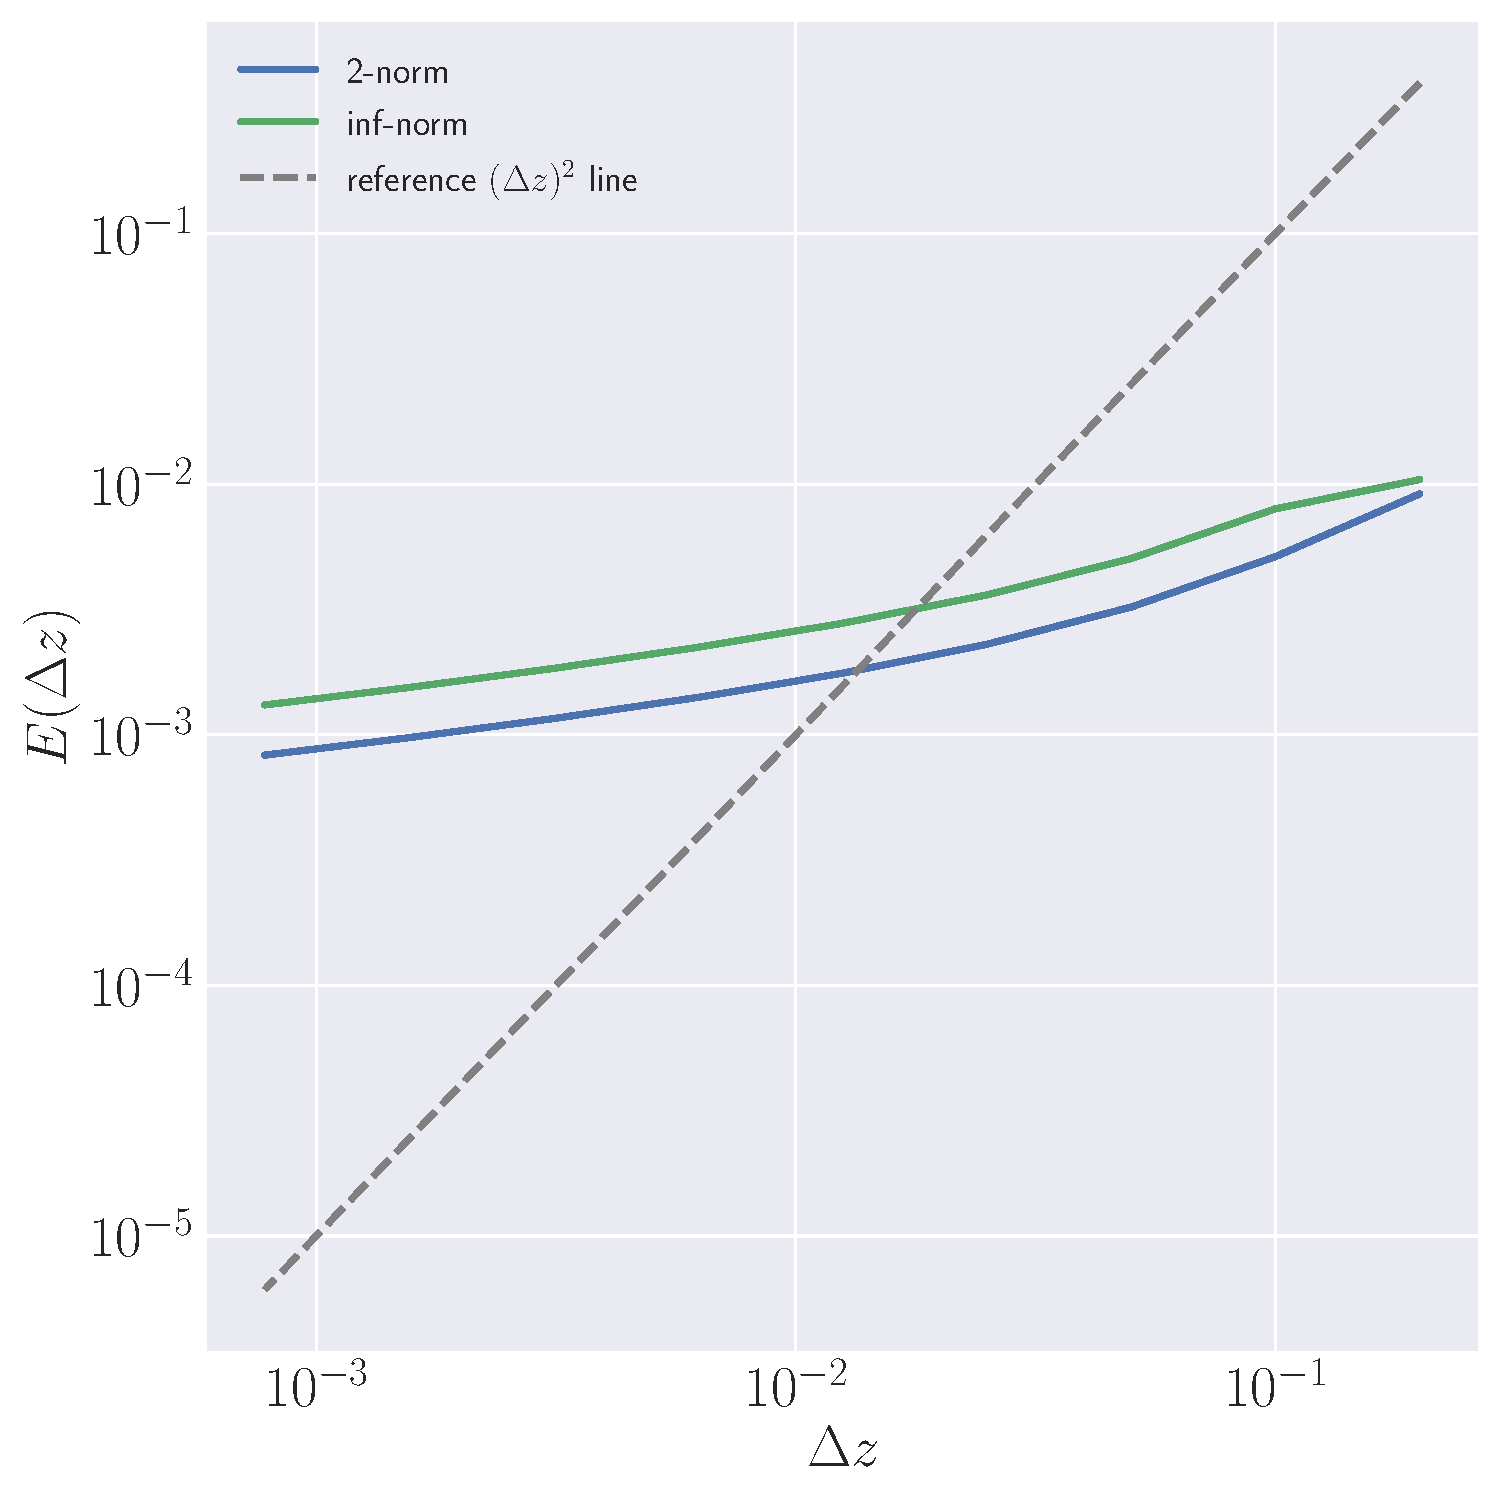
\includegraphics[clip, scale=0.40]{q2d_fig.pdf}
	\caption{Problem 2, part D. Error as a function of \emph{uniform grid} spacing. }
\end{figure}

\section*{Problem 3}

\subsection*{Part A}
So we are given the the following boundary value problem
\begin{align}
    u^{\prime\prime}(x)-8xu(x) = -4x^{2},\ -2 < x <1;\ u(-2) = -1,\ u^{\prime}(1) = \dfrac{1}{2}.
\end{align}
To solve numerically we have to discretize this problem. We utilize a uniform grid,
\begin{align}
    x_{i} = -2 + ih,\ i = 0,\dots,m+1
\end{align}
of step size $h = \frac{3}{m+1}$ where $m$ is the number of internal grid points.
Let $U_{i} = u(x_{i})$ as usual. We use the centered-difference scheme for the second derivative:
\begin{subequations}
    \begin{align}
        \left(\dfrac{U_{i-1}-2U_{i}+U_{i+1}}{h^{2}}\right) - 8x_{i}U_{i} &= -4x_{i}^{2}\\
        \left(\dfrac{U_{i-1}-2U_{i}+U_{i+1}}{h^{2}}\right) - \dfrac{8h^{2}\left(-2+ih\right)U_{i}}{h^{2}} &= -4(-2+ih)^{2}\\
        \dfrac{1}{h^{2}}\left[U_{i-1}-2\left(1-8h^{2}+4ih^{3}\right)U_{i}+U_{i+1}\right] &= -4\left(4-4ih+i^{2}h^{2}\right)\\
        \dfrac{1}{h^{2}}\left[U_{i-1}-2\left(1-8h^{2}+4ih^{3}\right)U_{i}+U_{i+1}\right] &= -16+16ih-4i^{2}h^{2}\\
        \dfrac{1}{h^{2}}\left[U_{i-1}-2\left(1-8h^{2}+4ih^{3}\right)U_{i}+U_{i+1}\right] &= 16\left(ih-1\right)-4i^{2}h^{2}.
    \end{align}
\end{subequations}
Casting this in the form of $A\vb{U}=\vb{F}$ we have
\begin{align}
    \dfrac{1}{h^{2}}\begin{pmatrix}
        1 & 0 & 0 & \cdots & \cdots & \cdots & 0\\
        1 & g_{1} & 1 & 0 & \cdots & \cdots &0 \\
        0 & 1 & g_{2} & 1 & 0 & \cdots & 0 \\
        0 & 0 & \ddots & \ddots & \ddots & 0 & 0 \\
        0 & \cdots & 0 & \ddots & \ddots & \ddots & 0  \\
        0 & \cdots & \cdots & 0 & 1 & g_{m} & 1\\
        0 & \cdots & \cdots & \cdots & \cdots & -1 & 1\\
    \end{pmatrix}
    \begin{pmatrix}
        u_{0} \\ u_{1} \\ u_{2} \\ \vdots \\ \vdots \\ u_{m} \\ u_{m+1}
    \end{pmatrix}
    =
    \begin{pmatrix}
        f_{0} \\ f_{1} \\ f_{2} \\ \vdots \\ \vdots \\ f_{m} \\ f_{m+1}
    \end{pmatrix}
\end{align}
where the diagonals of the internal matrix are $g_{i} = -2(1-8h^{2}+4ih^{3})$, and the forcing terms on the right-hand side are
\begin{align}
    f_{i} =
    \begin{cases}
        -\nicefrac{1}{h^{2}},&\quad i = 0\\
        16(ih-1)-4i^{2}h^{2},&\quad i=1,\dots,m\\
        \nicefrac{1}{2h},&\quad i = m+1
    \end{cases}
\end{align}
In this case the solution is linear since the particular solution of this ODE is given by the form $u_{p}(x) = ax$.
Substituting this into the differential equation we solve for the coefficient $a$
\begin{subequations}
    \begin{align}
        u_{p}^{\prime\prime}(x) - 8xu_{p}(x) &= -4x^{2}\\
        -8ax^{2} &= -4x^{2} \\
        \implies a &= \dfrac{1}{2},
    \end{align}
\end{subequations}
and therefore the particular solution is given by
\begin{align}
    u_{p}(x) = \dfrac{1}{2}x
\end{align}

\begin{figure}[!h]
	\centering
	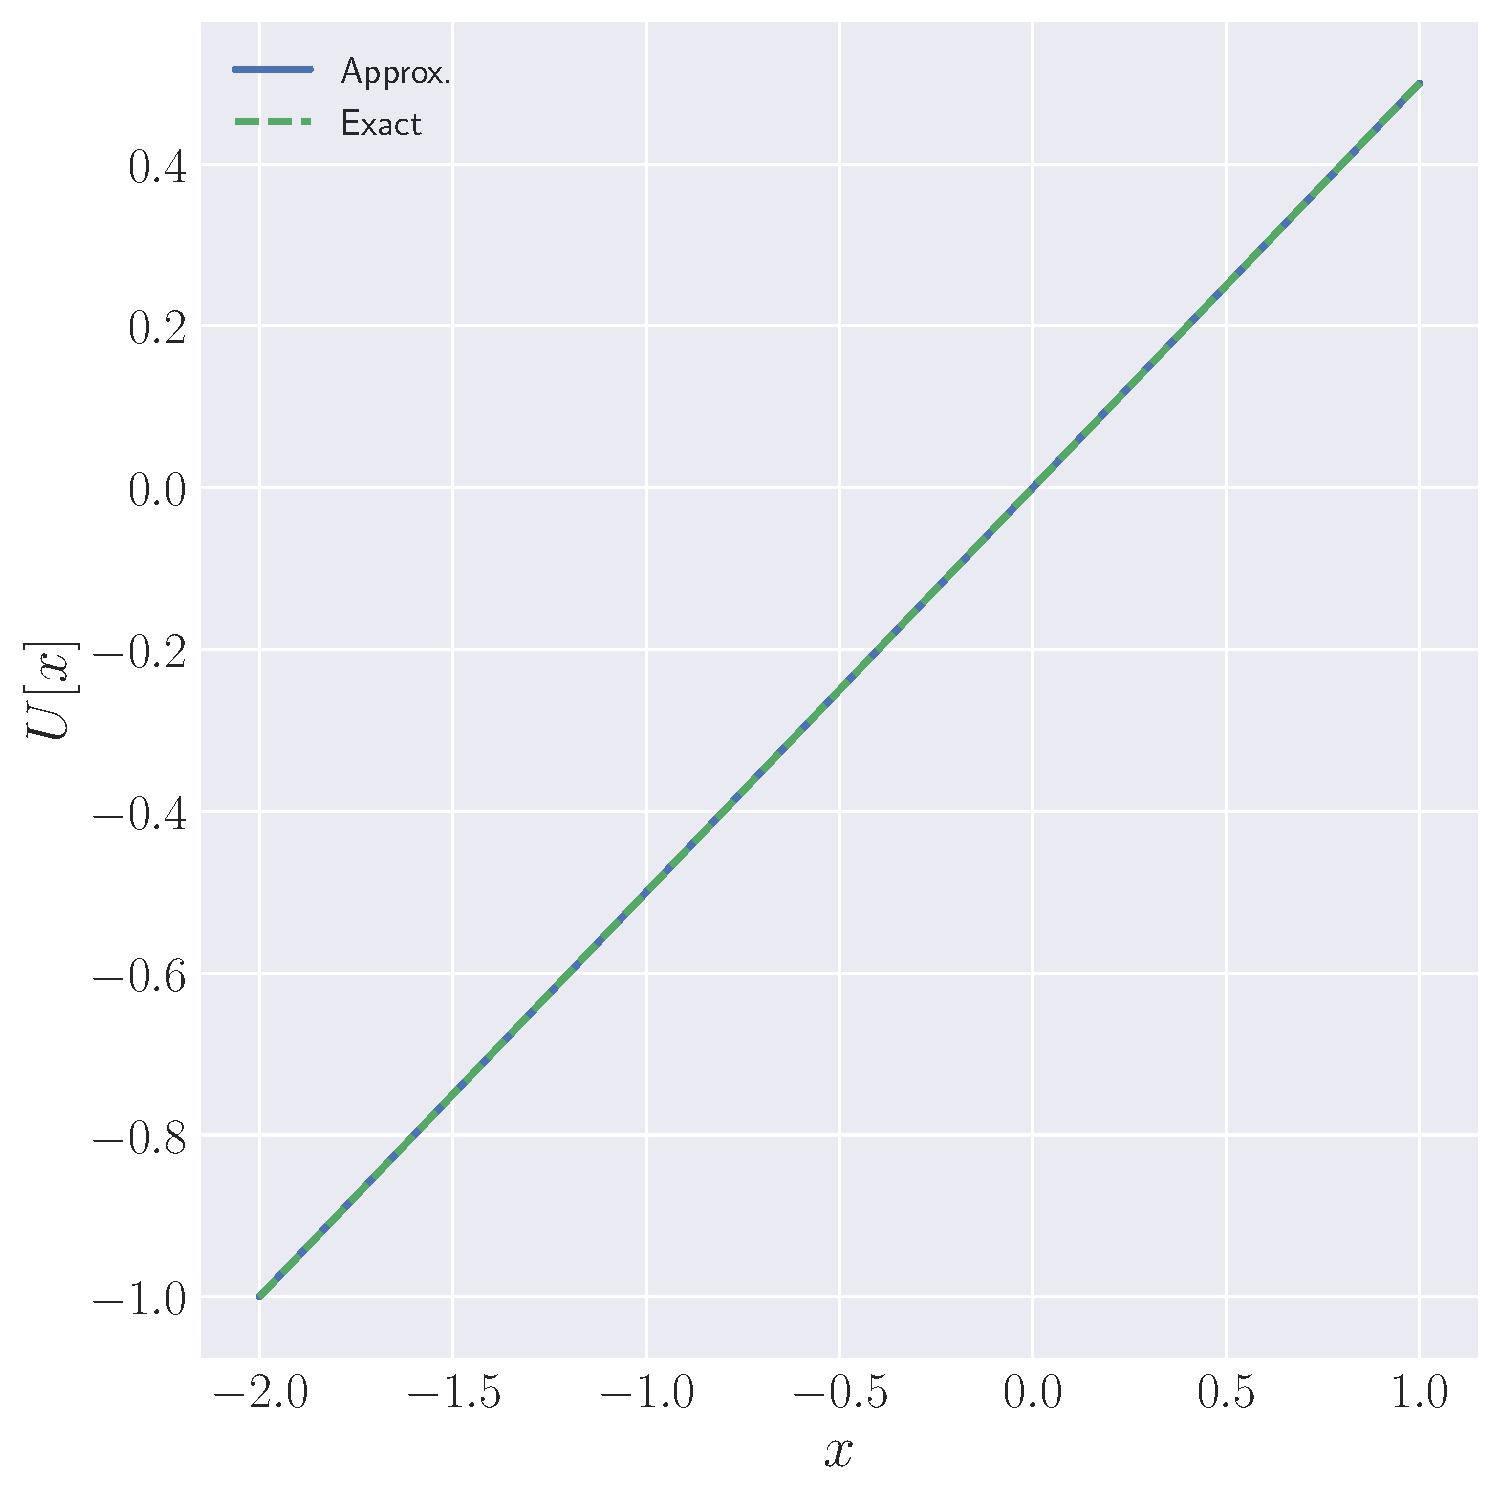
\includegraphics[clip, scale=0.30]{q3a_fig.pdf}
	\caption{Problem 3, part A. Approximate solution $U[x]$ as a function of $x$. Particular solution of ODE plotted as reference.}
\end{figure}

\FloatBarrier

\subsection*{Part B}

\begin{figure}[!h]
	\centering
	\subfloat{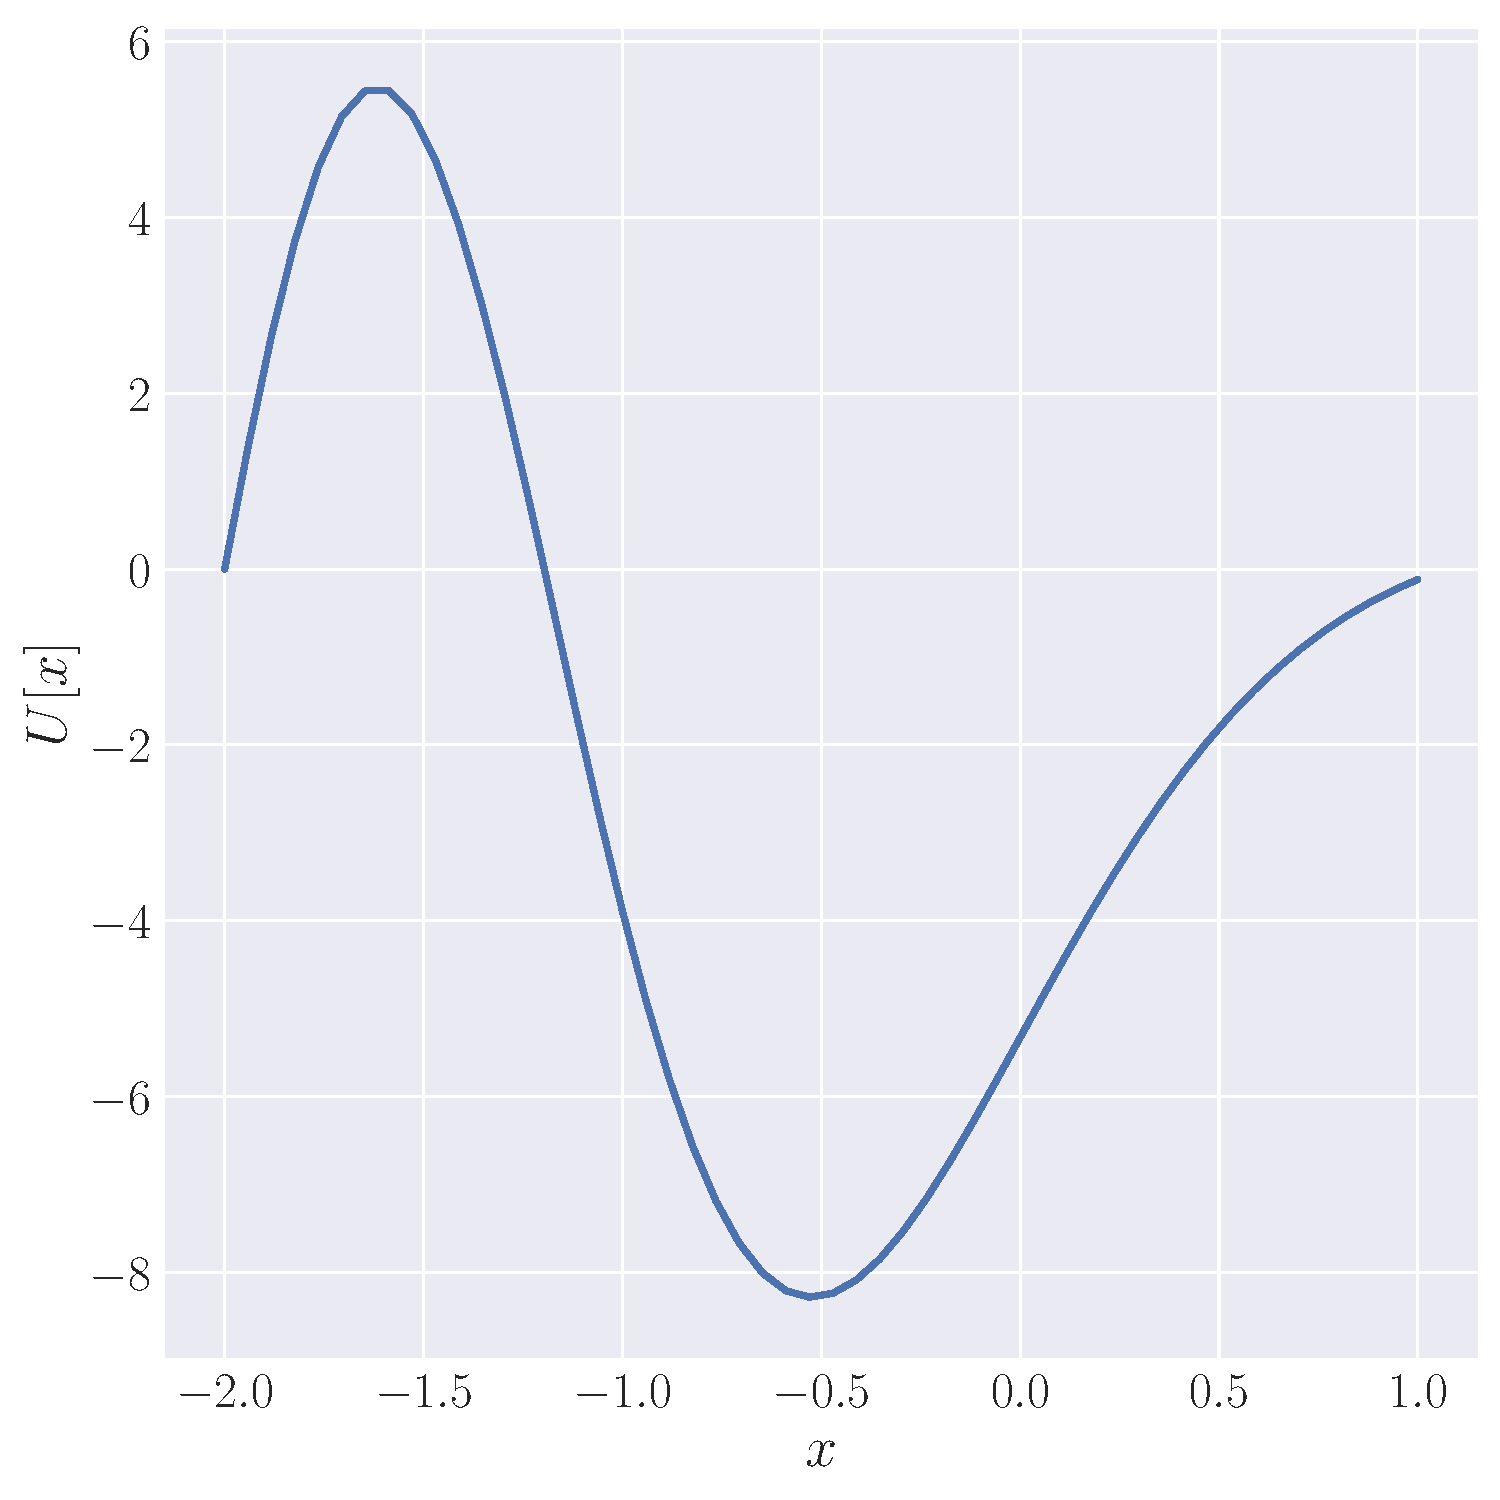
\includegraphics[clip, scale=0.30]{q3b_sample_fig.pdf}}
	\subfloat{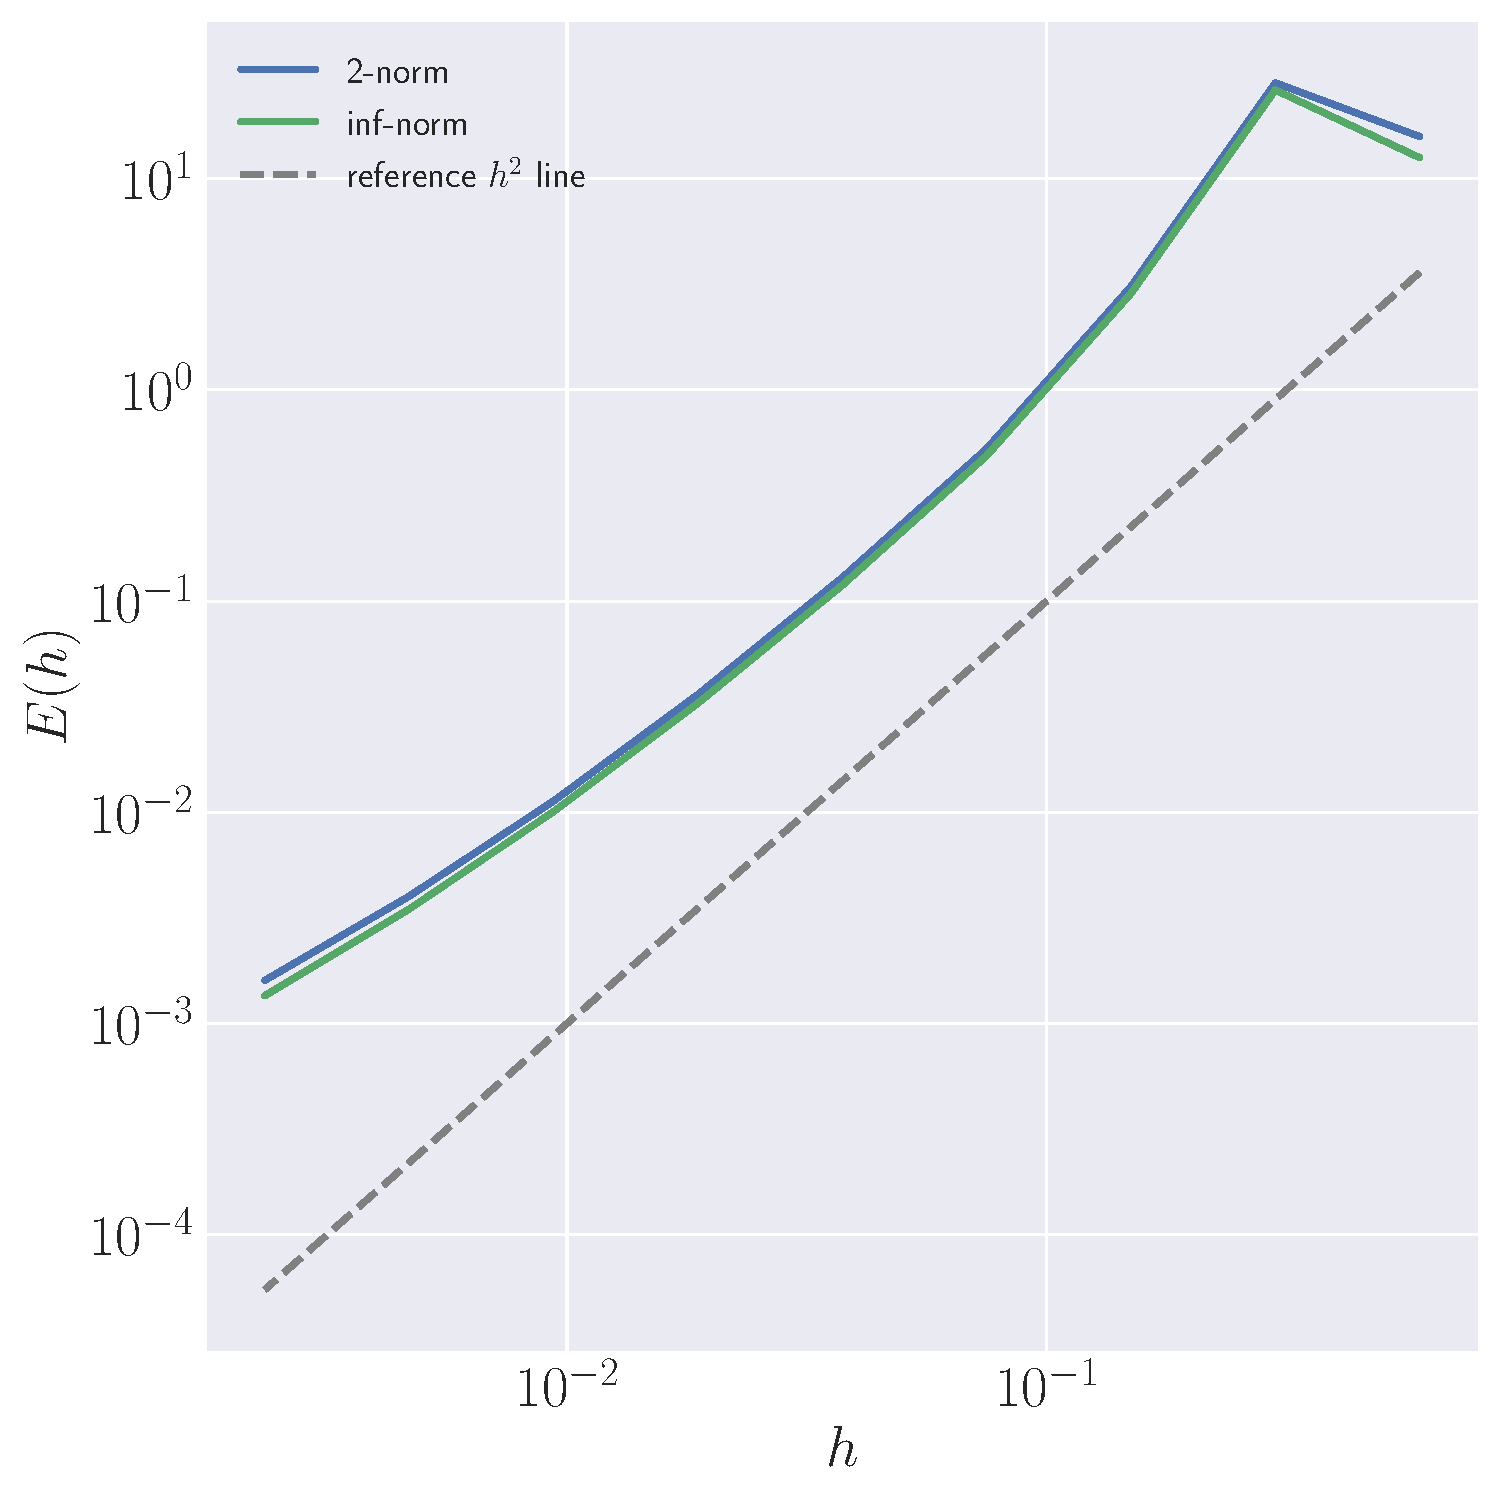
\includegraphics[clip, scale=0.30]{q3b_part1_fig.pdf}}

	\subfloat{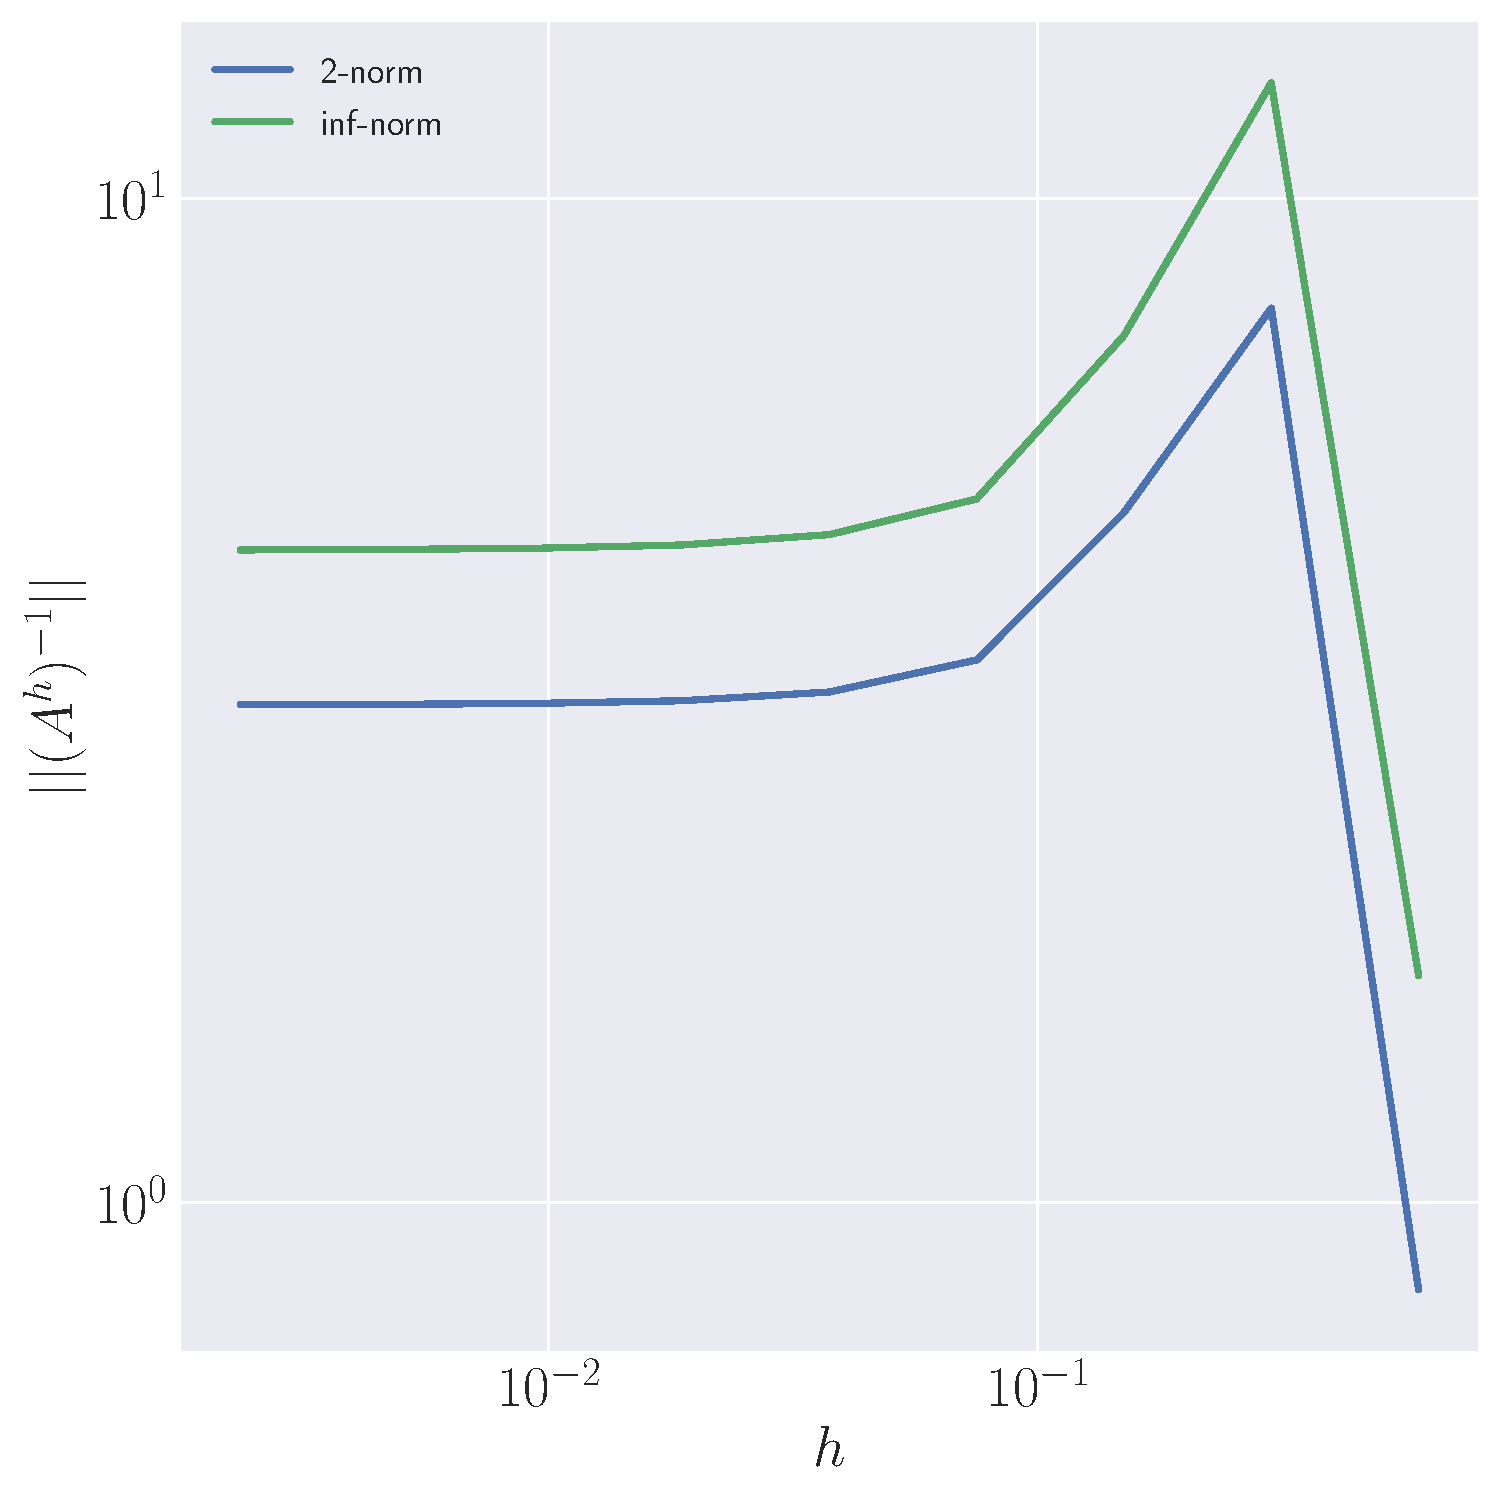
\includegraphics[clip, scale=0.30]{q3b_part2_fig.pdf}}
	\caption{
		Problem 3, part B. [Top left-hand subplot] Approximate solution $U[x]$ as a function of $x$. [Top left-hand subplot] Error in the approximate solution vector $E(h)$ as a function of step-size $h$. Different colors for the 2-norm (blue) and the inf-norm (green). Dashed grey line is $E(h) = h^{2}$ for reference. [Bottom subplot] Induced matrix norm of $(A^{h})^{-1}$ as a function of step-size $h$.
	}
\end{figure}


\FloatBarrier

\subsection*{Part C}

If we use a centered difference at the right-hand end point then we acquire the equation
\begin{subequations}
    \begin{align}
        u^{\prime}(1) &\approx \dfrac{u(1+h)-u(1-h)}{2h}\\
        2 &= \dfrac{U_{m+2}-U_{m}}{2h},
    \end{align}
\end{subequations}
which implies that the ``ghost point'' $U_{m+2}$ is
\begin{align}
    U_{m+2} = U_{m} + 4h.
\end{align}
Now, assert that the differential equation also holds on the boundary
\begin{subequations}
    \begin{align}
        f(1) &\approx  \dfrac{U_{m+2}-2U_{m+1}+U_{m}}{h^{2}} - \dfrac{8x_{m+1}h^{2}U_{m+1}}{h^{2}},\\
        &= \dfrac{1}{h^{2}}\left[U_{m+2}-(2+8h^{2})U_{m+1}+U_{m}\right]
    \end{align}
\end{subequations}

and put the two equations together
\begin{subequations}
    \begin{align}
        \dfrac{U_{m+2}-2U_{m+1}+U_{m}}{h^{2}} &= \dfrac{\left(4h + U_{m}\right)-(2+8h^{2})U_{m+1}+U_{m}}{h^{2}}\\
        f(1) &= \dfrac{4}{h} + \dfrac{2}{h^{2}}U_{m} - \dfrac{2+8h^{2}}{h^{2}}U_{m+1}\\
        &= \dfrac{4}{h} + \dfrac{2}{h^{2}}\left[U_{m}-(1+4h^{2})U_{m+1}\right]\\
        \implies (1+4h^{2})U_{m+1}-U_{m} &= 2(1+h)
    \end{align}
\end{subequations}
Therefore, to acquire second order accuracy, the following modifications must be made to the matrix $A$ and the forcing term:
\begin{align}
\dfrac{1}{h^{2}}\begin{pmatrix}
1 & 0 & 0 & \cdots & \cdots & \cdots & 0\\
1 & g_{1} & 1 & 0 & \cdots & \cdots &0 \\
0 & 1 & g_{2} & 1 & 0 & \cdots & 0 \\
0 & 0 & \ddots & \ddots & \ddots & 0 & 0 \\
0 & \cdots & 0 & \ddots & \ddots & \ddots & 0  \\
0 & \cdots & \cdots & 0 & 1 & g_{m} & 1\\
0 & \cdots & \cdots & \cdots & \cdots & -1 & 1+4h^{2}\\
\end{pmatrix}
\begin{pmatrix}
u_{0} \\ u_{1} \\ u_{2} \\ \vdots \\ \vdots \\ u_{m} \\ u_{m+1}
\end{pmatrix}
=
\begin{pmatrix}
f_{0} \\ f_{1} \\ f_{2} \\ \vdots \\ \vdots \\ f_{m} \\ f_{m+1}
\end{pmatrix}
\end{align}
\begin{align}
    f_{i} =
    \begin{cases}
        -\nicefrac{1}{h^{2}},&\quad i = 0\\
        16(ih-1)-4i^{2}h^{2},&\quad i=1,\dots,m\\
        \nicefrac{2+2h}{h},&\quad i = m+1
    \end{cases}
\end{align}

\begin{figure}[!h]
	\centering
	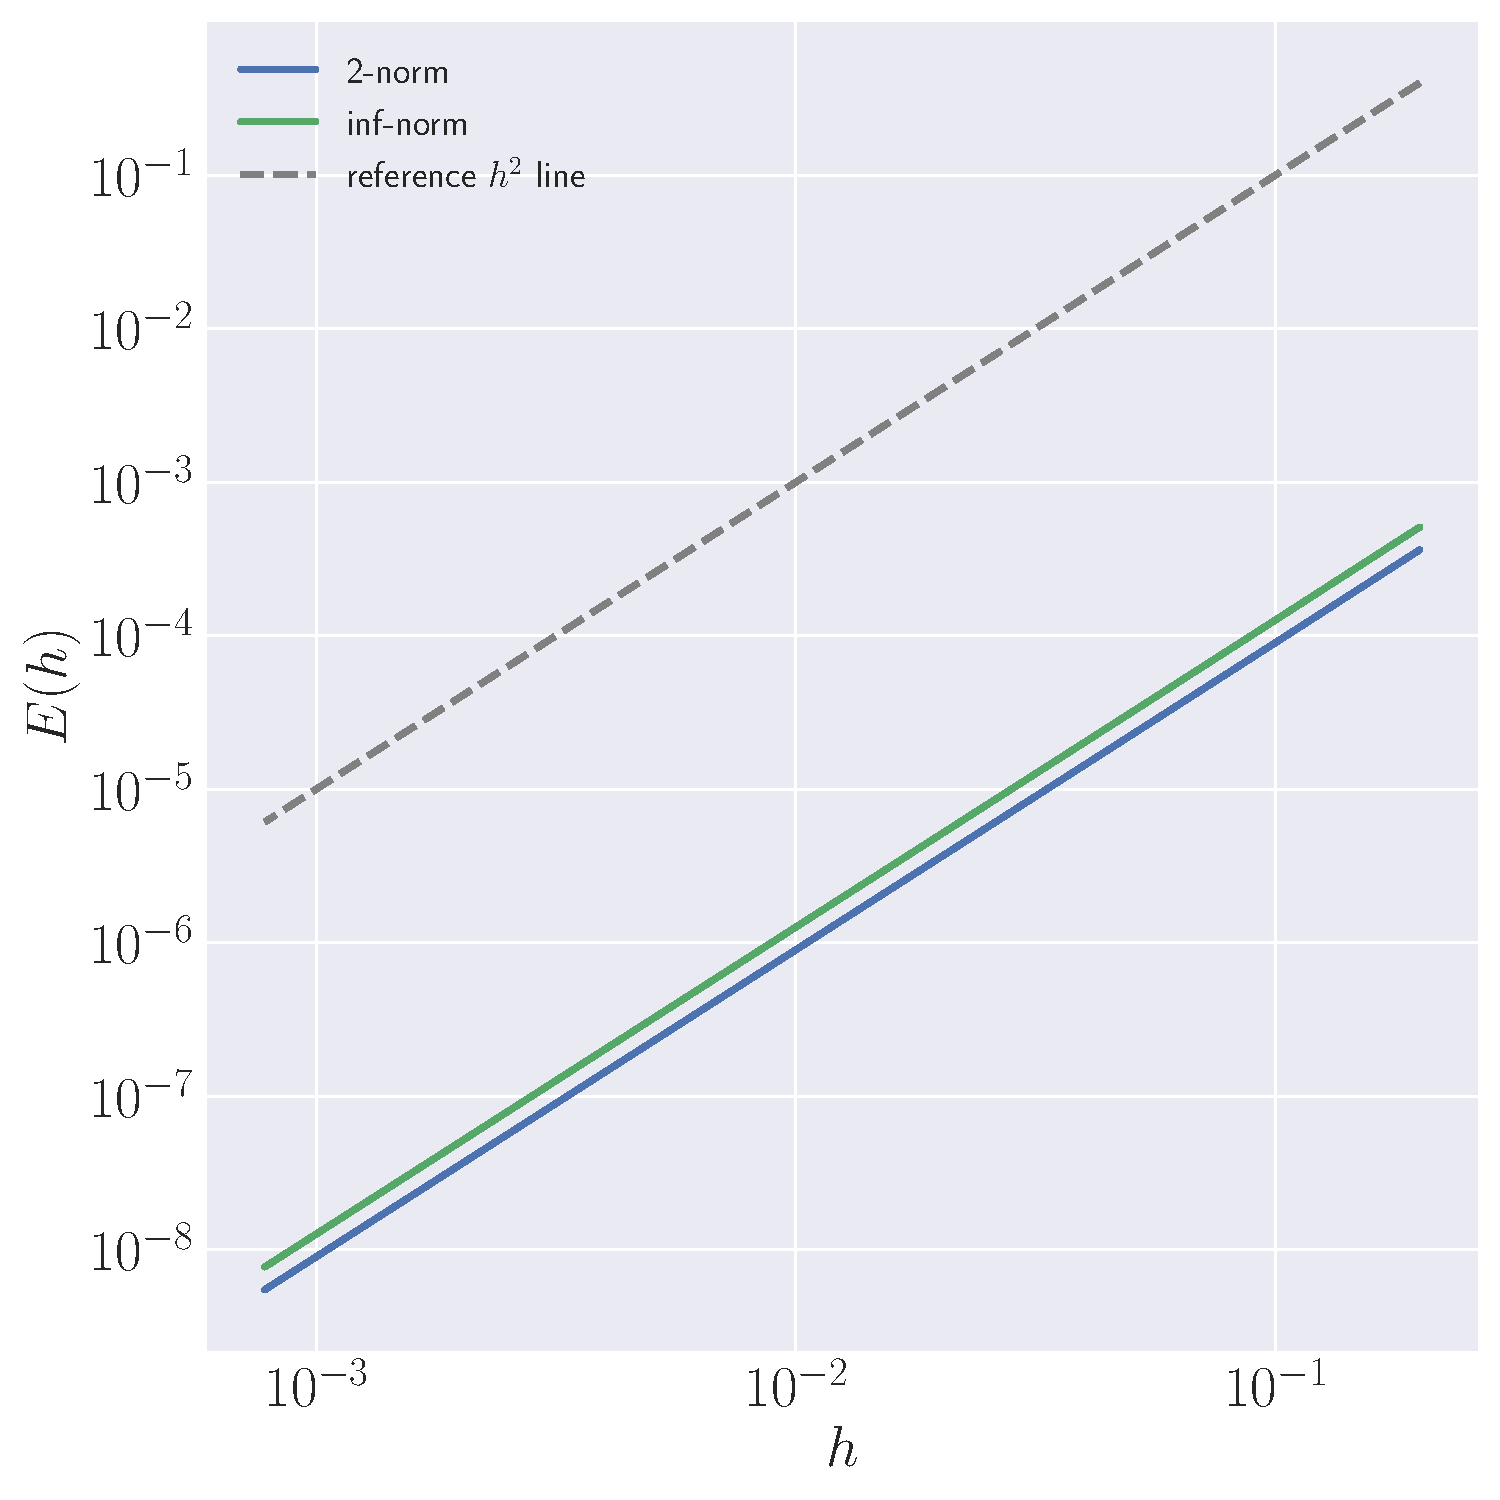
\includegraphics[clip, scale=0.40]{q3c_fig.pdf}
	\caption{
		Problem 3, part C. Error in the approximate solution vector $E(h)$ as a function of step-size $h$. Different colors for the 2-norm (blue) and the inf-norm (green). Dashed grey line is $E(h) = h^{2}$ for reference.
	}
\end{figure}

\subsection*{Part D}
If we use a one-sided approximation to $u^{\prime}(x_{m+1}=1)$ then we have
\begin{subequations}
    \begin{align}
         \dfrac{1}{2h}\left[3U_{m+1}-4U_{m}+U_{m-1}\right]  \approx u^{\prime}(1) &= 2\\
         \dfrac{1}{h^{2}}\left[3U_{m+1}-4U_{m}+U_{m-1}\right] &= \dfrac{4}{h}.
    \end{align}
\end{subequations}
Therefore, to acquire second order accuracy, the following modifications must be made to the matrix $A$ and the forcing term:
\begin{align}
    \dfrac{1}{h^{2}}
    \begin{pmatrix}
        1 & 0 & 0 & \cdots & \cdots & \cdots & 0\\
        1 & g_{1} & 1 & 0 & \cdots & \cdots &0 \\
        0 & 1 & g_{2} & 1 & 0 & \cdots & 0 \\
        0 & 0 & \ddots & \ddots & \ddots & 0 & 0 \\
        0 & \cdots & 0 & \ddots & \ddots & \ddots & 0  \\
        0 & \cdots & \cdots & 0 & 1 & g_{m} & 1\\
        0 & \cdots & \cdots & \cdots & 1 & -4 & 3\\
    \end{pmatrix}
    \begin{pmatrix}
        U_{0} \\ U_{1} \\ U_{2} \\ \vdots \\ \vdots \\ U_{m} \\ U_{m+1}
    \end{pmatrix}
    =
    \begin{pmatrix}
        f_{0} \\ f_{1} \\ f_{2} \\ \vdots \\ \vdots \\ f_{m} \\ f_{m+1}
    \end{pmatrix}
\end{align}
\begin{align}
    f_{i} =
    \begin{cases}
        -\nicefrac{1}{h^{2}},&\quad i = 0\\
        16(ih-1)-4i^{2}h^{2},&\quad i=1,\dots,m\\
        \nicefrac{4}{h},&\quad i = m+1
    \end{cases}
\end{align}

\begin{figure}[!h]
	\centering
	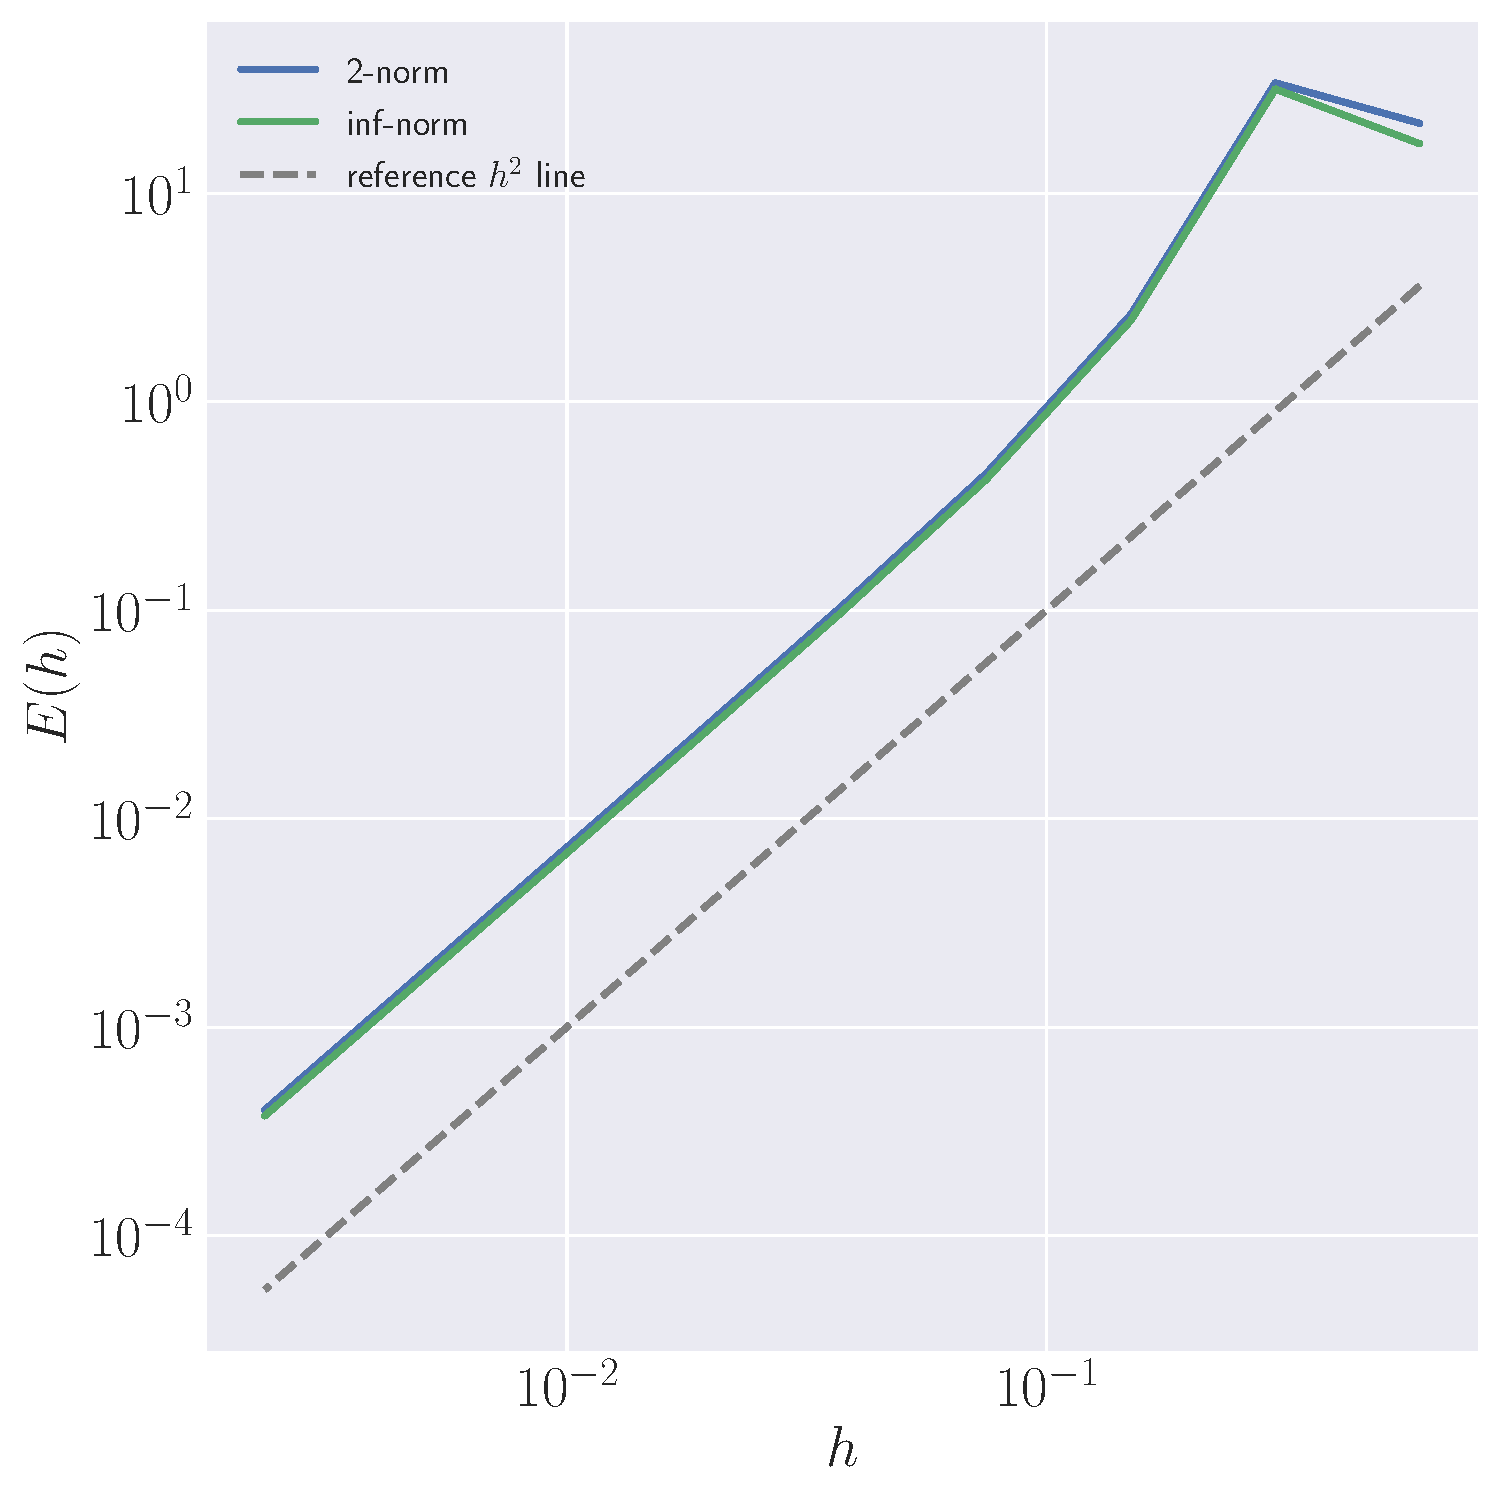
\includegraphics[clip, scale=0.40]{q3d_fig.pdf}
	\caption{
		Problem 3, part D. Error in the approximate solution vector $E(h)$ as a function of step-size $h$. Different colors for the 2-norm (blue) and the inf-norm (green). Dashed grey line is $E(h) = h^{2}$ for reference.
	}
\end{figure}

\FloatBarrier

\section*{Problem 4}

\subsection*{Part A}

We first solve the homogeneous case. Propose the solution
\begin{align}
	y(x) = Ae^{\lambda x}.
\end{align}
Substituting into the homogeneous differential equation gives
\begin{align}
	\lambda(\varepsilon\lambda + 1) = 0.
\end{align}
Thus the homogeneous case is
\begin{align}
	y_{c} = Ae^{-x/\varepsilon} + B.
\end{align}
For the particular solution we guess a particular solution of the form
\begin{align}
	y_{p} = Ce^{-x}.
\end{align}
Substitute into the differential equation to acquire
\begin{subequations}
	\begin{align}
		C-1 &= e^{-1},\\
		\implies C &= 1+e
	\end{align}
\end{subequations}
Thus the full solution is given by
\begin{align}
	y(x) = Ae^{-x/\varepsilon} + (1-e)e^{-x} + B.
\end{align}
However, if $\varepsilon = 1$ then, the complementary and particular solutions become linearly dependent. In this case, to return the orthogonality of the two solutions we have that
\begin{align}
	y(x) = Ae^{-x} + (1-e)xe^{-x} + B
\end{align}
Applying the boundary conditions to these two solutions separately we have then that
\begin{align}
    \hspace{-1cm}y(x) =
    \begin{cases}
	    -\dfrac{e^{1-x}}{e-1}\left[e^{x}+x-ex-1\right],&\quad \varepsilon = 1\\
	    \dfrac{e^{-x}}{(\varepsilon-1) \left(e^{\nicefrac{1}{\varepsilon}}-1\right)} \left[ e^{\frac{1+\varepsilon x}{\varepsilon}}-e^{\frac{(\varepsilon-1)x+1}{\varepsilon}}+e^{\frac{(\varepsilon-1)x+\varepsilon+1}{\varepsilon}}-e^{\frac{1+\varepsilon}{\varepsilon}}-e^{x+1}+e
	    \right],&\quad \mathrm{else}.\\
    \end{cases}
\end{align}

\subsection*{Part B}
Discretizing the BVP over a uniform grid
\begin{align}
    x_{i} = ih,\ i = 0, \dots, m+1
\end{align}
with $h = \frac{1}{m+1}$ yields the following:
\begin{subequations}
    \begin{align}
        -e^{1-x} &= \varepsilon y^{\prime\prime} + y^{\prime} \\
        &\approx \dfrac{\varepsilon}{h^{2}}\left[Y_{i+1}-2Y_{i}+Y_{i-1}\right] + \dfrac{1}{2h}\left[Y_{i+1}-Y_{i-1}\right]\\
        &= \dfrac{1}{2h^{2}}\left[(2\varepsilon+h)Y_{i+1}-4\varepsilon Y_{i} + (2\varepsilon-h)Y_{i-1}\right].
    \end{align}
\end{subequations}
Thus this gives a system of equations that can be cast into the form $A\vb{U} = \vb{F}$,
\begin{align}
    \dfrac{1}{2h^{2}}
    \begin{pmatrix}
    1 & 0 & 0 & \cdots & \cdots & \cdots & 0\\
    (2\varepsilon - h) & -4\varepsilon & (2\varepsilon + h) & 0 & \cdots & \cdots &0 \\
    0 & (2\varepsilon - h) & -4\varepsilon & (2\varepsilon + h) & 0 & \cdots & 0 \\
    0 & 0 & \ddots & \ddots & \ddots & 0 & 0 \\
    0 & \cdots & 0 & \ddots & \ddots & \ddots & 0  \\
    0 & \cdots & \cdots & 0 & (2\varepsilon - h) & -4\varepsilon & (2\varepsilon + h)\\
    0 & \cdots & \cdots & \cdots & 0 & 0 & 1\\
    \end{pmatrix}
    \begin{pmatrix}
    Y_{0} \\ Y_{1} \\ Y_{2} \\ \vdots \\ \vdots \\ Y_{m} \\ Y_{m+1}
    \end{pmatrix}
    =
    \begin{pmatrix}
    f_{0} \\ f_{1} \\ f_{2} \\ \vdots \\ \vdots \\ f_{m} \\ f_{m+1}
    \end{pmatrix}
\end{align}
with
\begin{align}
    f_{i} =
    \begin{cases}
        0,&\quad i = 0\\
        -e^{1-ih},&\quad i=1,\dots,m\\
        0,&\quad i = m+1
    \end{cases}
\end{align}

\begin{figure}[!h]
	\centering
	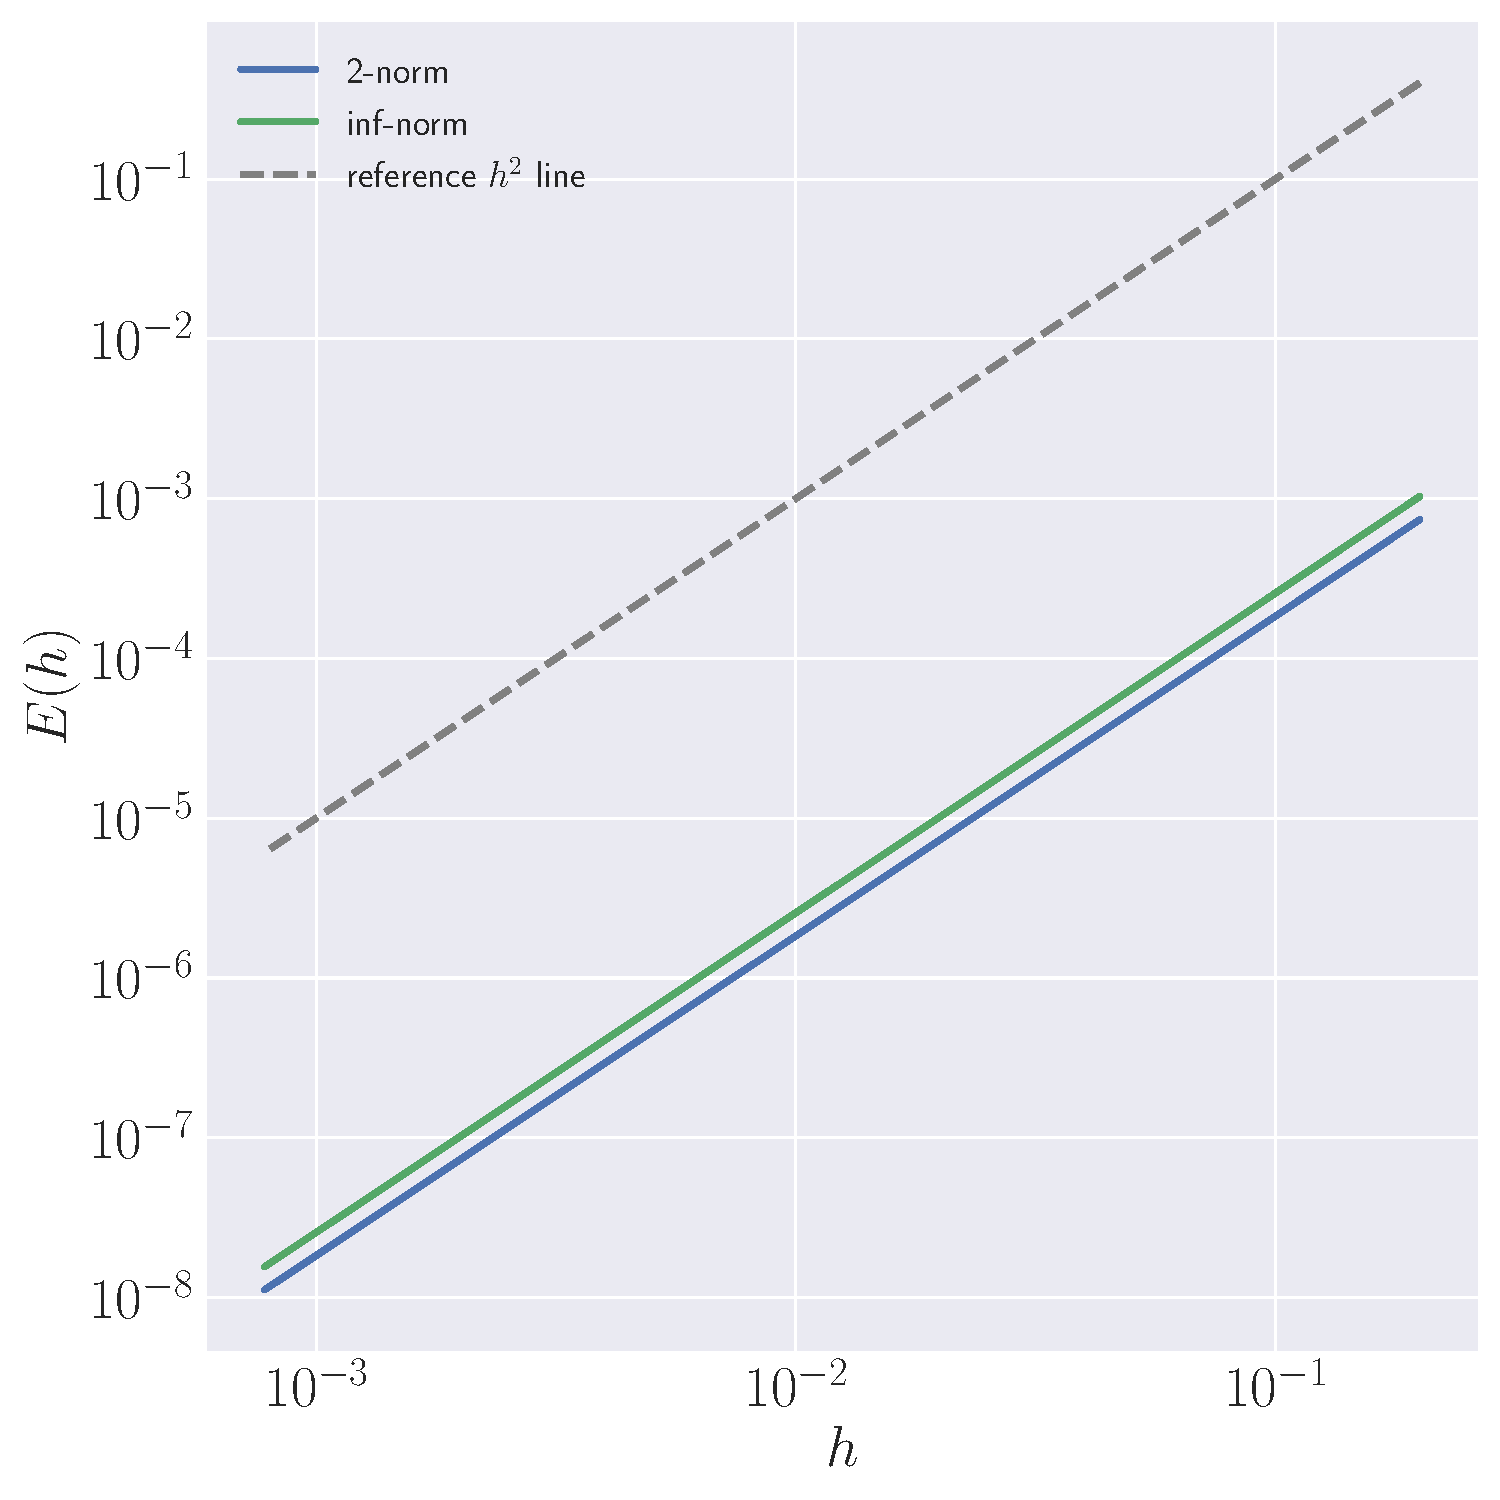
\includegraphics[clip, scale=0.40]{q4b_fig.pdf}
	\caption{
		Problem 4, part B. Error in the approximate solution vector $E(h)$ as a function of step-size $h$. Different colors for the 2-norm (blue) and the inf-norm (green). Dashed grey line is $E(h) = h^{2}$ for reference.
	}
\end{figure}

\subsection*{Part C}
Implementing the method of deferred corrections, we modify the right hand side from
\begin{align}
    f(x) \to f(x) + \dfrac{h^{2}}{12}f^{\prime\prime}(x).
\end{align}
Thus we have that the RHS needs to modified to
\begin{align}
    f_{i} =
    \begin{cases}
        0,&\quad i = 0\\
        -\dfrac{e^{1-ih}}{12}(12+h^{2}),&\quad i=1,\dots,m\\
        0,&\quad i = m+1
    \end{cases}
\end{align}

\subsection*{Part D}
Let $U_{i} = u(ih)$ be the coarse solution, $V_{i} = u(ih/2)$ be the solution on the finer grid, and $W_{i} = u(ih/4)$ be the solution on
the very fine grid. Since we have a second-order method, the error for each of these functions is given by :
\begin{align}
U_{i} - u(ih) &= c_{2}h^{2} + c_{4}h^{4} + c_{6}h^{6} + \mathrm{h.o.t}
\end{align}
\begin{subequations}
    \begin{align}
        V_{2i} - u(ih) &= c_{2}\left(\dfrac{h}{2}\right)^{2} + c_{4}\left(\dfrac{h}{2}\right)^{4} + c_{6}\left(\dfrac{h}{2}\right)^{6} + \mathrm{h.o.t}\\
        &= \dfrac{c_{2}}{4}h^{2} + \dfrac{c_{4}}{16}h^{4} + \dfrac{c_{6}}{64}h^{6} + \mathrm{h.o.t}
    \end{align}
\end{subequations}
\begin{subequations}
    \begin{align}
        W_{4i} - u(ih) &= c_{2}\left(\dfrac{h}{4}\right)^{2} + c_{4}\left(\dfrac{h}{4}\right)^{4} + c_{6}\left(\dfrac{h}{4}\right)^{6} + \mathrm{h.o.t}\\
        &= \dfrac{c_{2}}{16}h^{2} + \dfrac{c_{4}}{256}h^{4} + \dfrac{c_{6}}{4096}h^{6} + \mathrm{h.o.t}
    \end{align}
\end{subequations}
The most accurate solution estimate using these values will be sixth-order accurate. Having an arbitrary linear combination
\begin{align}
    a(W_{4i}-u(ih)) + b(V_{2i}-u(ih)) + \gamma(U_{i}-u(ih)) &= aW_{4i} + bV_{2i} + \gamma U_{i} - (a+b+\gamma)u(ih).
\end{align}
Equivalently, we have that
\begin{subequations}
    \begin{align}
        \hspace{-1cm} a(W_{4i}-u(ih)) + b(V_{2i}-u(ih)) + \gamma(U_{i}-u(ih)) &= a\left[\dfrac{c_{2}}{16}h^{2} + \dfrac{c_{4}}{256}h^{4}\right] + b\left[\dfrac{c_{2}}{4}h^{2} + \dfrac{c_{4}}{16}h^{4} \right] + \gamma\left[c_{2}h^{2} + c_{4}h^{4}\right]\\
        &= \left(\dfrac{a}{16}+\dfrac{b}{4}+\gamma\right)c_{2}h^{2}
        + \left(\dfrac{a}{256}+\dfrac{b}{16}+\gamma\right)c_{4}h^{4} + \mathrm{h.o.t}.
    \end{align}
\end{subequations}
Imposing that the first two-error terms have to be zero and additionally,
imposing that $a + b + c = 1$, then we have the system of equations
\begin{align}
	\begin{bmatrix}
		\frac{1}{16} & \frac{1}{4} & 1\\
		\frac{1}{256} & \frac{1}{16} & 1\\
		1 & 1 & 1
	\end{bmatrix}
	\begin{bmatrix}
		a \\ b \\ c
	\end{bmatrix}
	=
	\begin{bmatrix}
		0 \\ 0 \\ 1
	\end{bmatrix}
\end{align}
which yields the solution
\begin{subequations}
	\begin{align}
		a &= \dfrac{64}{45}\\
		b &= -\dfrac{4}{9}\\
		\gamma &= \dfrac{1}{45}.
	\end{align}
\end{subequations}
Therefore the linear combination that gives the deferred corrections is
\begin{align}
	\dfrac{64}{45}W_{4i} - \dfrac{4}{9}V_{2i} + \dfrac{1}{45}U_{i}
\end{align}

\begin{figure}[!h]
	\centering
	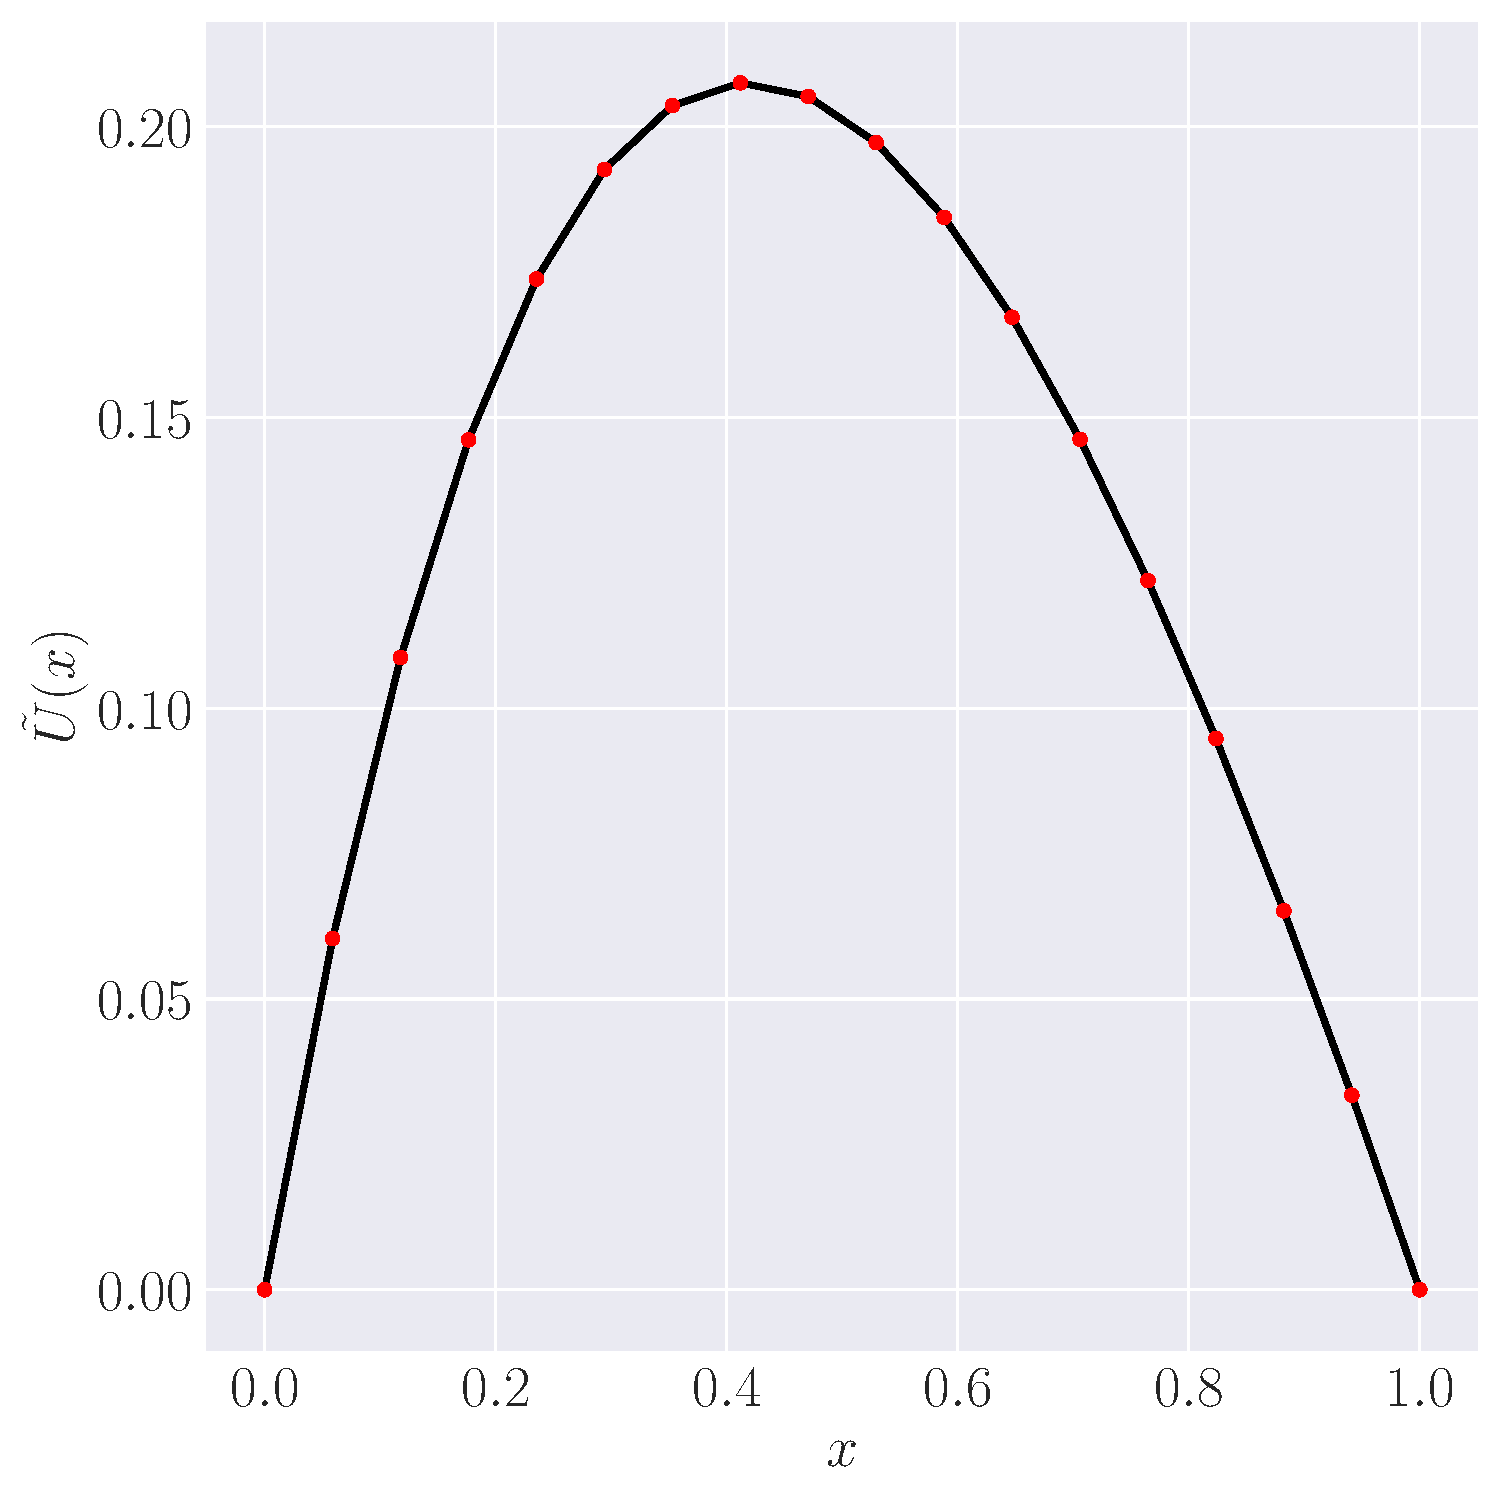
\includegraphics[clip, scale=0.30]{q4d_fig.pdf}
	\caption{
		Problem 4, part D. Approximate solution $U[x]$, acquired from deferred corrections, as a function of $x$.
	}
\end{figure}

\subsection*{Part E}

We observe (Fig.~\ref{fig:p4e}) that unless the boundary layer is well-resolved, the method does not converge to the correct solution

\begin{figure}[!h]
	\centering
	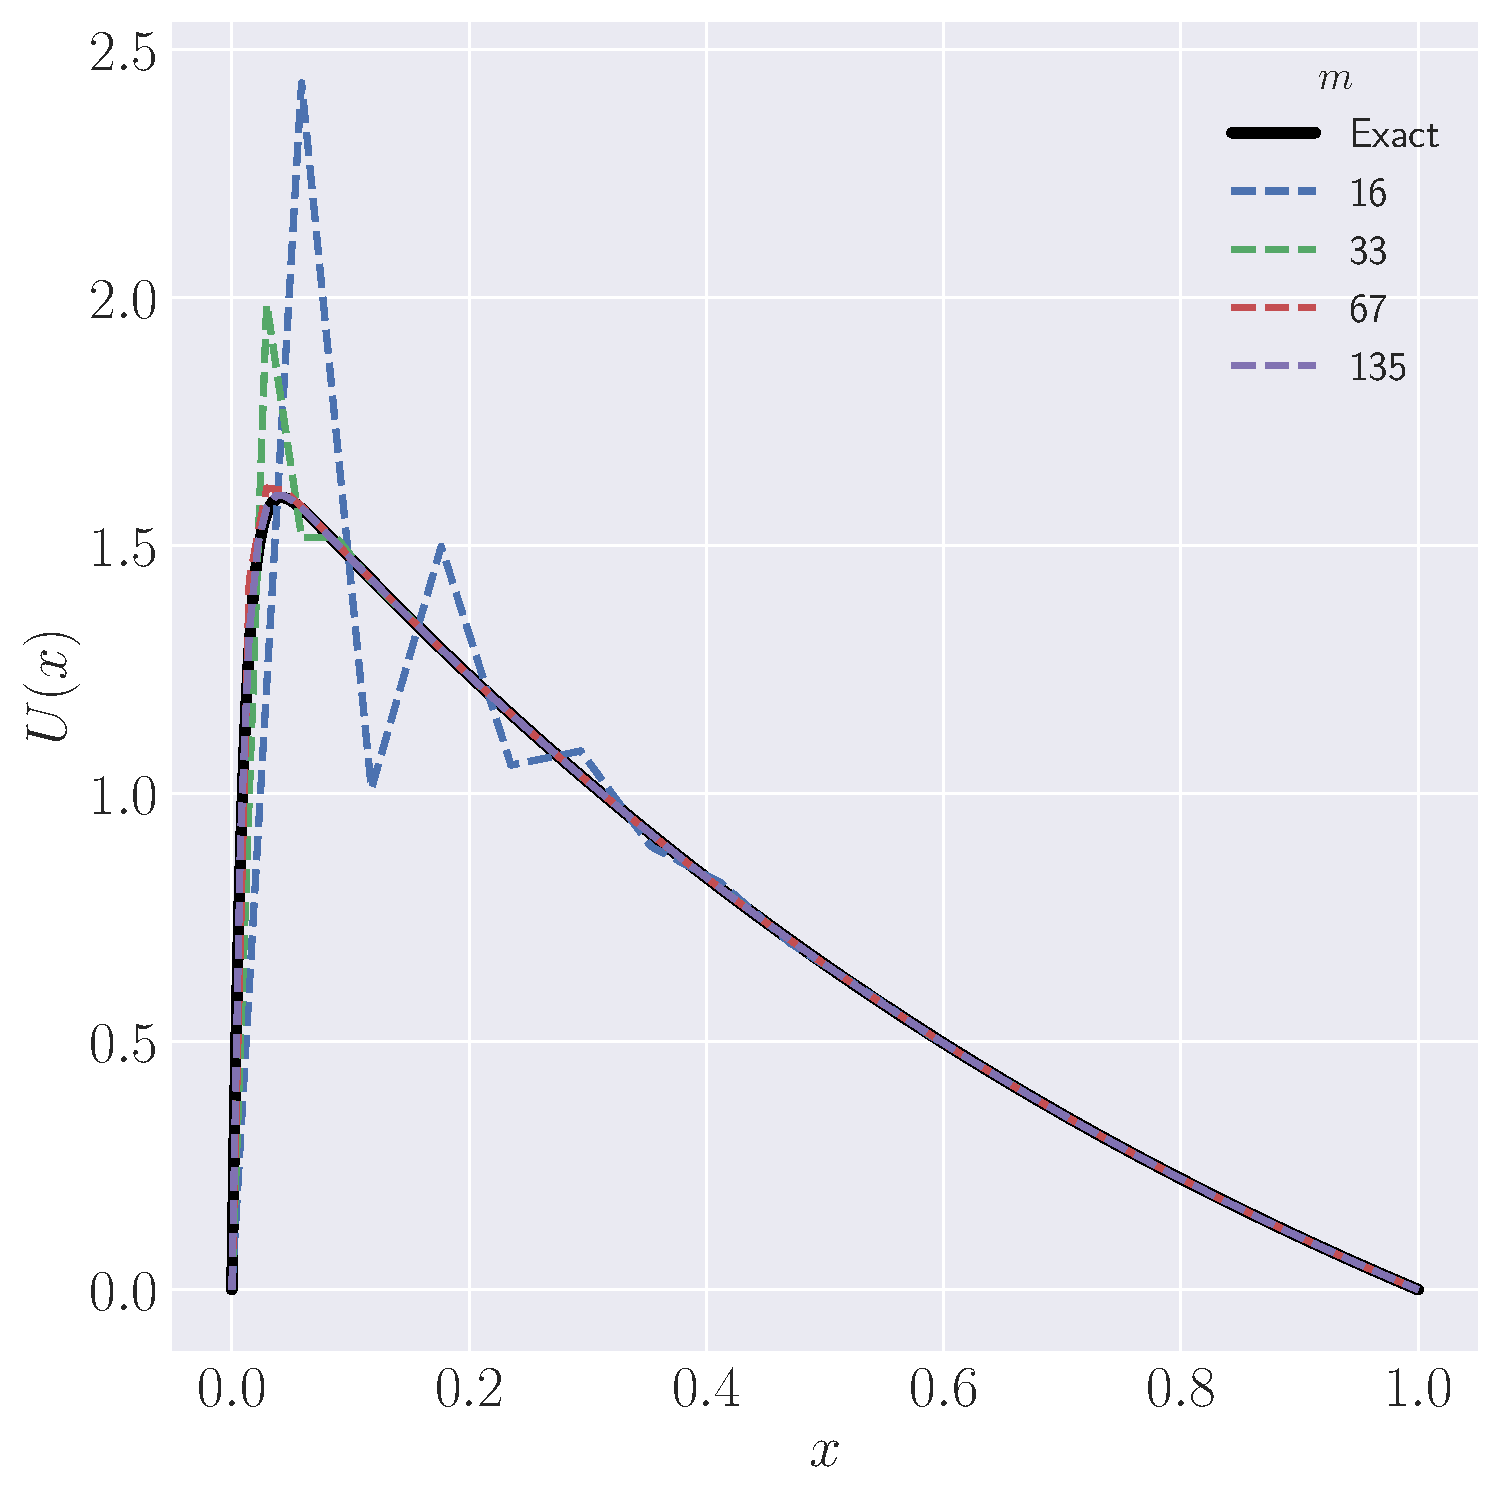
\includegraphics[clip, scale=0.30]{q4e_fig.pdf}
	\caption{
		Problem 4, part E. Approximate solution $U[x]$ as a function of $x$. Different colors denote different numbers of \emph{internal} mesh points. Exact solution in black for reference.
	}
	\label{fig:p4e}
\end{figure}

\end{document}